% ===================== PREAMBLE =====================
\documentclass[10pt,twoside]{article}
\usepackage[T1]{fontenc}
\usepackage[utf8]{inputenc}
\usepackage{mathpazo}
\usepackage{amssymb}
\usepackage{microtype}
\usepackage[letterpaper,top=0.85in,bottom=0.95in,left=0.85in,right=0.85in]{geometry}
\usepackage{xcolor}
\usepackage{tikz}
\usetikzlibrary{positioning,shadows,shapes.geometric,shapes.misc,calc,arrows.meta,fit,backgrounds,decorations.pathmorphing}
\usepackage[most]{tcolorbox}
\usepackage{multicol}
\usepackage{enumitem}
\usepackage{titlesec}
\usepackage{fancyhdr}
\usepackage{wrapfig}
\usepackage{graphicx}
\usepackage{array}
\usepackage{needspace}
\usepackage{longtable}
\usepackage[hidelinks]{hyperref}

% ---------- palette ----------
\definecolor{templegreen}{HTML}{1E3A2F}
\definecolor{moss}{HTML}{3B5741}
\definecolor{bloodred}{HTML}{7B1113}
\definecolor{darkred}{HTML}{4E0C0D}
\definecolor{bone}{HTML}{EFE7D4}
\definecolor{parch}{HTML}{FBF6E8}
\definecolor{stone}{HTML}{4A4A44}
\definecolor{gold}{HTML}{9A7B34}
\definecolor{sewage}{HTML}{5C5A2E}
\definecolor{faceless}{HTML}{2A2333}

\hypersetup{colorlinks=true,linkcolor=darkred,urlcolor=bloodred}

% ---------- headers/footers ----------
\pagestyle{fancy}
\fancyhf{}
\renewcommand{\headrulewidth}{0.6pt}
\renewcommand{\footrulewidth}{0pt}
\fancyhead[LE]{\small\scshape\textcolor{bloodred}{The Lost Temple of Cazic--Thule}}
\fancyhead[RO]{\small\scshape\textcolor{bloodred}{\leftmark}}
\fancyfoot[C]{\small\textcolor{stone}{\thepage}}

% ---------- section styling ----------
\titleformat{\section}
  {\normalfont\Large\bfseries\scshape\color{bloodred}}
  {\thesection}{0.8em}{}[{\color{bloodred}\titlerule[1.2pt]}]
\titleformat{\subsection}
  {\normalfont\large\bfseries\scshape\color{templegreen}}
  {\thesubsection}{0.6em}{}
\titleformat{\subsubsection}
  {\normalfont\normalsize\bfseries\color{darkred}}
  {}{0em}{}

% ---------- ability score line ----------
\newcommand{\abilities}[6]{%
\begin{center}\small
\setlength{\tabcolsep}{6pt}\renewcommand{\arraystretch}{1.05}
\begin{tabular}{cccccc}
\textbf{STR}&\textbf{DEX}&\textbf{CON}&\textbf{INT}&\textbf{WIS}&\textbf{CHA}\\[1pt]
#1&#2&#3&#4&#5&#6\\
\end{tabular}\end{center}}

% red divider used inside stat blocks
\newcommand{\sbrule}{\par\vspace{2pt}\noindent{\color{bloodred}\rule{\linewidth}{1.1pt}}\par\vspace{2pt}}

% ---------- STAT BLOCK ----------
\newtcolorbox{statblock}[1]{%
  breakable, enhanced, colback=parch, colframe=bloodred,
  boxrule=1pt, arc=1.5pt, left=7pt, right=7pt, top=4pt, bottom=6pt,
  fonttitle=\bfseries\scshape\large, coltitle=parch, colbacktitle=bloodred,
  title={#1},
  before skip=8pt, after skip=8pt,
  overlay unbroken and first={\draw[bloodred,line width=1pt]
     ([xshift=2pt,yshift=-1pt]title.south west)--([xshift=-2pt,yshift=-1pt]title.south east);}
}

% ---------- ITEM CARD ----------
\newtcolorbox{itemcard}[2]{%
  breakable, enhanced, colback=bone, colframe=templegreen,
  boxrule=1pt, arc=2pt, left=7pt, right=7pt, top=4pt, bottom=6pt,
  fonttitle=\bfseries\scshape\large, coltitle=parch, colbacktitle=templegreen,
  title={#1}, before skip=8pt, after skip=8pt,
  after title={\hfill\normalfont\itshape\small #2}
}

% ---------- READ-ALOUD (boxed text) ----------
\newtcolorbox{readaloud}{%
  breakable, enhanced, colback=parch!70!white, colframe=stone,
  boxrule=0.6pt, arc=1pt, left=10pt, right=10pt, top=6pt, bottom=6pt,
  borderline west={2.5pt}{0pt}{bloodred},
  fontupper=\itshape, before skip=8pt, after skip=8pt
}

% ---------- DM / DESIGN NOTE ----------
\newtcolorbox{dmnote}[1][Running It]{%
  breakable, enhanced, colback=templegreen!8!white, colframe=templegreen,
  boxrule=0.6pt, arc=1pt, left=8pt,right=8pt,top=4pt,bottom=5pt,
  fonttitle=\bfseries\scshape, coltitle=parch, colbacktitle=templegreen,
  title={#1}, before skip=8pt, after skip=8pt
}

% ---------- technical room key ----------
\newtcolorbox{techbox}{%
  enhanced, colback=stone!7!white, colframe=stone!55!black,
  boxrule=0.5pt, arc=1pt, left=7pt,right=7pt,top=3pt,bottom=4pt,
  before skip=6pt, after skip=8pt, fontupper=\small
}

\newcommand{\tech}[1]{\textbf{\scshape\textcolor{stone}{#1}}\ }

% quick tags
\newcommand{\CR}[1]{\textnormal{(CR #1)}}
\newcommand{\eqname}[1]{\textsc{#1}}
\setlist[itemize]{leftmargin=1.3em,itemsep=1pt,topsep=2pt}
\setlist[enumerate]{leftmargin=1.5em,itemsep=1pt,topsep=2pt}

\linespread{1.03}
\begin{document}

% ============================================================ TITLE
\thispagestyle{empty}
\begin{center}
\vspace*{0.4in}

\begin{tikzpicture}[scale=1]
  \fill[templegreen] (-2.6,0) -- (2.6,0) -- (1.9,0.7) -- (-1.9,0.7) -- cycle;
  \fill[templegreen] (-1.9,0.7) -- (1.9,0.7) -- (1.2,1.4) -- (-1.2,1.4) -- cycle;
  \fill[templegreen] (-1.2,1.4) -- (1.2,1.4) -- (0.55,2.15) -- (-0.55,2.15) -- cycle;
  % the Hands of Cazic-Thule rising from the apex (severed at the wrist)
  \fill[bone] (-0.5,2.15) .. controls (-0.62,2.7) and (-0.55,3.05) .. (-0.4,3.2)
     -- (-0.28,3.15) -- (-0.28,3.35) -- (-0.14,3.38) -- (-0.14,3.15)
     -- (0.0,3.15) -- (0.0,3.4) -- (0.14,3.4) -- (0.14,3.12)
     -- (0.3,3.05) .. controls (0.5,2.9) and (0.5,2.5) .. (0.5,2.15) -- cycle;
  \draw[gold,line width=1pt] (-2.9,-0.16)--(2.9,-0.16);
\end{tikzpicture}

\vspace{0.35in}
{\scshape\color{stone}\large A Fifth Edition Descent}\\[0.15in]
{\Huge\bfseries\scshape\color{bloodred} The Lost Temple\\[2pt] of Cazic--Thule}\\[0.16in]
{\scshape\color{templegreen}\normalsize Being an account of the Alliz Tae Ew,\\ their sleeping god, and the price of a broken oath}\\[0.22in]
{\itshape\color{templegreen}\large ``The weak, they will eat. So say I, and so it is.''}\\[0.35in]

\begin{minipage}{0.82\textwidth}\centering\small\color{stone}
An adventure in the drowned Feerrott, for four to six characters of \textbf{5th to
11th level} (optimized for \textbf{8th}). A living god-city of blind, cannibal
lizardfolk, their captive kin, the planar horrors that slipped through a rift in
the world, and the Sleeping Watcher who waits beneath the pyramid to be woken by a
gong.
\end{minipage}

\vfill
{\footnotesize\color{stone}
An unofficial homage to the classic \textit{EverQuest} zone. Cazic--Thule, the
Alliz Tae Ew, the Avatar of Fear, Tool Haslick, and the Feerrott are creations of
the \textit{EverQuest} universe (here converted to 5e and adapted from Project 1999
lore and the in-world texts ``Tales of the Alliz Ew'' and the tale of Vashahkti).
Not for sale.\par}
\vspace{0.2in}
\end{center}
\clearpage

% ============================================================ HOW TO USE
\section*{How To Use This Book}
\addcontentsline{toc}{section}{How To Use This Book}
\markboth{How To Use This Book}{How To Use This Book}

This is a single mega-dungeon: not a corridor of encounters, but a \emph{city} that
happens to be underground and consecrated to terror. The old faithful still live
here --- blind, cannibal, and certain. They breed, they cook (one another, when the
weak falter), they bury their dead in the ossuary, they bicker over rank, and above
all they feed the thing beneath the pyramid so that it will keep sleeping. The
players are trespassers in a working temple whose landlord is a god.

The book has three layers so you can run it your way:
\begin{itemize}
\item \textbf{The narrative body} describes each of five districts as a living
place: who lives there, what they want, what the rooms smell like, and how the
quests thread through them.
\item \textbf{Technical room keys} (gray boxes) give the crunch: dimensions, light,
exits, DCs, and hazards.
\item \textbf{The Appendices} hold every monster and treasure as a standalone card.
\end{itemize}

\begin{dmnote}[A Note on the Tongue]
The lizardfolk language (rendered here from the Rallosian, as the in-world
translator Pearl Honeywine did) is old Common turned back-to-front. \emph{Alliz} is
``zilla'' reversed --- lizard. \emph{Ew} is ``we.'' \emph{Tae} is ``eat.''
\emph{Evol} is ``love.'' So the two great clans name themselves plainly if you read
them backward: the \textbf{Alliz Tae Ew} are the ones who say \emph{``we eat,''} and
their despised cousins the \textbf{Alliz Evol Ew} are the ones who say \emph{``we
love.''} Players who notice will unlock half the setting's menace on their own; drop
the hint and let them.
\end{dmnote}

\begin{dmnote}[On Canon and Level]
In the original zone the temple's denizens run levels 19--45; this conversion
deliberately down-scales the whole city to challenge an 8th-level party, treating
the temple as it was \emph{felt} on a first low-level venture rather than as its
literal high-level self. Every canonical faction, guardian, and relic is present ---
just tuned down. To run it at its true weight, roughly double monster hit points and
add +3 to save DCs and attack bonuses.
\end{dmnote}

\begin{dmnote}[The Feeling You Want]
Cazic--Thule is the god of \emph{fear}, not gore. The temple should feel watched.
The carved hands turn to follow the party. The Tae Ew, blind from the rituals of
darkness, ``see'' by scent and sound and the taste of terror on the air. Lean on
dread and ritual and the sense that the deepest room already knows their names.
\end{dmnote}
\clearpage

% ============================================================ HISTORY
\section*{The Truth Beneath the Temple}
\addcontentsline{toc}{section}{The Truth Beneath the Temple}
\markboth{The Truth Beneath the Temple}{The Truth Beneath the Temple}

In the long-ago, a lizardfolk patriarch named \eqname{Tool Haslick} channeled the
Lore of Fear and heard Cazic--Thule, the Faceless, speaking in his skull. The god
showed him a vision: a green plague that would dissolve his enemies' insides to
ooze, and a temple-city raised in the god's honor. Haslick became the first of his
race to eat the flesh of his own kind --- inspired, he said, by the Faceless
himself. His colony recoiled. So Haslick and those who followed him fled into the
swamp and founded a new tribe in a hidden temple: the \eqname{Alliz Tae Ew}, the
\emph{We Who Eat}. Their kin who refused --- the \eqname{Alliz Evol Ew}, the
\emph{We Who Love} --- remained in the Feerrott, and the two have hated each other
ever since.

The Tae Ew were cunning. They knew Cazic--Thule and his ilk would never suffer to
be worshipped second, so although in their hearts they also revered \eqname{Alliz
Onu, She Who Creates} --- the Queen --- they built the whole city as a temple to the
Faceless, a vast performance of devotion, so that the god would see their faith and
leave them free to worship as they pleased. Unwanted hatchlings and captured lesser
beings became the temple's servants and, when their purpose was done, its
sacrifices, their blood poured into the black stone Vessel at the god's altar.

Cazic--Thule was pleased. He reached down and blessed the Tae Ew with vigor, power,
and a bottomless blood-lust --- and in the reaching, a \textbf{rift} tore open
between the Plane of Fear and the waking world. Planar horrors flooded through it
into the temple and stayed, becoming its guardians: displaced, lethal, and loyal.
Some among the Tae Ew whispered that this was the fulfillment of Haslick's oldest
prophecy. Over the years the god's watch grew heavier; the priests took up
necromancy; the rites grew darker; and through dark portals they called yet more
things up out of the Plane of Fear.

Then the oath was broken. In the long-ago, Cazic--Thule and \eqname{Rallos Zek},
god of War, had clasped hands and sworn that neither god's army would defile the
other's temple. But the Rallosian host --- ogres, drunk on conquest and greedy for
the ``gemstones'' they imagined glittered within --- forgot the pact and stormed the
temple gates. They gloated over its treasures and poured Alliz Ew blood into the
sacred Vessel with no rite of purification, snapping off its handles in their
haste. The Tae Ew could only gnash their teeth and thrash their tails --- and wait.

They did not wait long. A young hatchling named \eqname{Vashahkti}, whose only duty
had been to wash the Vessel, fled to the inner sanctum and struck the great
\textbf{iron gong} so hard that it shattered and pierced him. The blow woke the
\eqname{Sleeping Watcher} --- the \textbf{Avatar of Fear}, Cazic's own shard given
flesh --- who thanked Vashahkti and made him the first sacrifice of the reckoning.
Days later came the \eqname{Green Dawn}: a cloud of pale green mist that fell upon
the Rallosian army and dissolved them where they stood, leaving them defeated and,
as the Tae Ew note with regret, \emph{inedible}.

The temple was ``lost'' to the world after that --- swallowed by vine and mist on
its swamp island. But it was never emptied. The congregation only grew stranger and
hungrier, and the Watcher, underfed for an age, sleeps ever more lightly.

\begin{dmnote}[Why the Party Is Here]
Pick or combine: (1) Feerrott villagers --- Evol Ew or ogre-kin --- have been taken
into the temple as servants and sacrifices; (2) a scholar hires the party to recover
a relic before a rival cult does; (3) captured mercenaries (a jailed dwarf, a band of
gnomish mages) have sent out a desperate message; (4) the swamp itself has begun to
\emph{whimper} at night, and druids fear the Watcher is finally waking.
\end{dmnote}

% ============================================================ FACTIONS
\section*{The Congregation: Factions}
\addcontentsline{toc}{section}{The Congregation}
\markboth{The Congregation}{The Congregation}

\subsection*{The Cazicite Priesthood (Tae Ew royalty and clergy)}
The ruling caste: templars, diviners, archons, cenobites --- the priest-kings of
the We Who Eat. They keep the Throne Room and the pyramids, wear the trappings of a
dead empire, and believe the temple's long decline is a test of faith to be met with
\emph{more} devotion, more sacrifice, more necromancy. Their patriarch,
\eqname{Tool Haslick} himself, is not dead so much as \emph{preserved} --- the first
cannibal, sustained past his time by the dark rites he pioneered. Proud, blind, and
utterly certain.

\subsection*{The Laity (common Alliz Tae Ew)}
The broad mass of the We Who Eat: broodlings, warders, pages, sentinels --- guards,
breeders, cooks, laborers, minor idol-keepers. They fill the Maze, the residential
warren, and mostly want to be left to their frightened, cannibal, ordinary lives.
All of them are blind, having given their sight to the rituals of darkness; all of
them will eat the weak among their own without a second thought. A clever party can
pass through the Maze by not \emph{acting} like prey or threat --- but these are not
sympathetic villagers, and the DM should resist making them so.

\subsection*{The Captives (Alliz Evol Ew and outsiders)}
The temple's servant-and-sacrifice underclass: captured \eqname{Alliz Evol Ew} ---
the We Who Love, sighted, hated cousins from the Feerrott --- alongside conquered
outsiders (a jailed dwarven mercenary, a cage of gnomish mages) and unwanted
hatchlings. Freeing them creates a second force inside the dungeon: a genuine ally,
though the Evol Ew have their own grievances and their own reasons to want the
temple burned. Killing temple denizens earns the party favor with the Feerrott
lizardfolk, and vice versa.

\subsection*{The Rift-Spawned (planar guardians)}
Not a faction so much as an infestation of loyalty. When Cazic blessed the Tae Ew, a
rift opened and things came through: \eqname{Fright}, \eqname{Terror}, and
\eqname{Dread} among them, displaced fear-elementals bound to the temple's defense.
Alongside them stand the priesthood's own constructs --- clay, stone, and steel
golems --- and the silvered guards. They do not eat, do not sleep, and do not tire.

\subsection*{The Faceless (Cazic--Thule) and the Queen}
The god is present in every carved absence-of-a-face, in the great severed
\textbf{Hands} at the temple's heart, and above all in the \textbf{Avatar of Fear}
sleeping in its green shell beneath the pyramid. Beneath the official devotion runs a
quieter current: the hidden worship of \eqname{Alliz Onu}, the Queen, She Who
Creates --- the tribe's true and secret love. A party that grasps this tension has a
lever the priesthood would kill to keep hidden.

\begin{dmnote}[The Dread Meter (optional)]
Keep a hidden \emph{Dread} score, starting at 0. It rises by 1 whenever the party
flees an encounter, fails a save against a fear effect, or witnesses a sacrifice at
the Vessel; it falls by 1 when they free captives, destroy an idol, or overcome a
named guardian. Several encounters scale with Dread. At Dread 6+, the Sleeping
Watcher stirs early and the whole temple grows tense and hostile.
\end{dmnote}
\clearpage

% ============================================================ MAP
\section*{General Map of the God-City}
\addcontentsline{toc}{section}{General Map}
\markboth{General Map}{General Map}

The temple is a multi-level warren on a swamp island, entered through a flooded
\textbf{Well} up from the Feerrott. This adventure organizes its sprawl into five
districts by function; the canonical camps (Courtyard ``CY,'' Throne Room ``TR,''
the two Pyramids, the Sewers, the Gator Pit) are noted where they fall. North is up;
solid arrows climb, dashed arrows descend.

\begin{center}
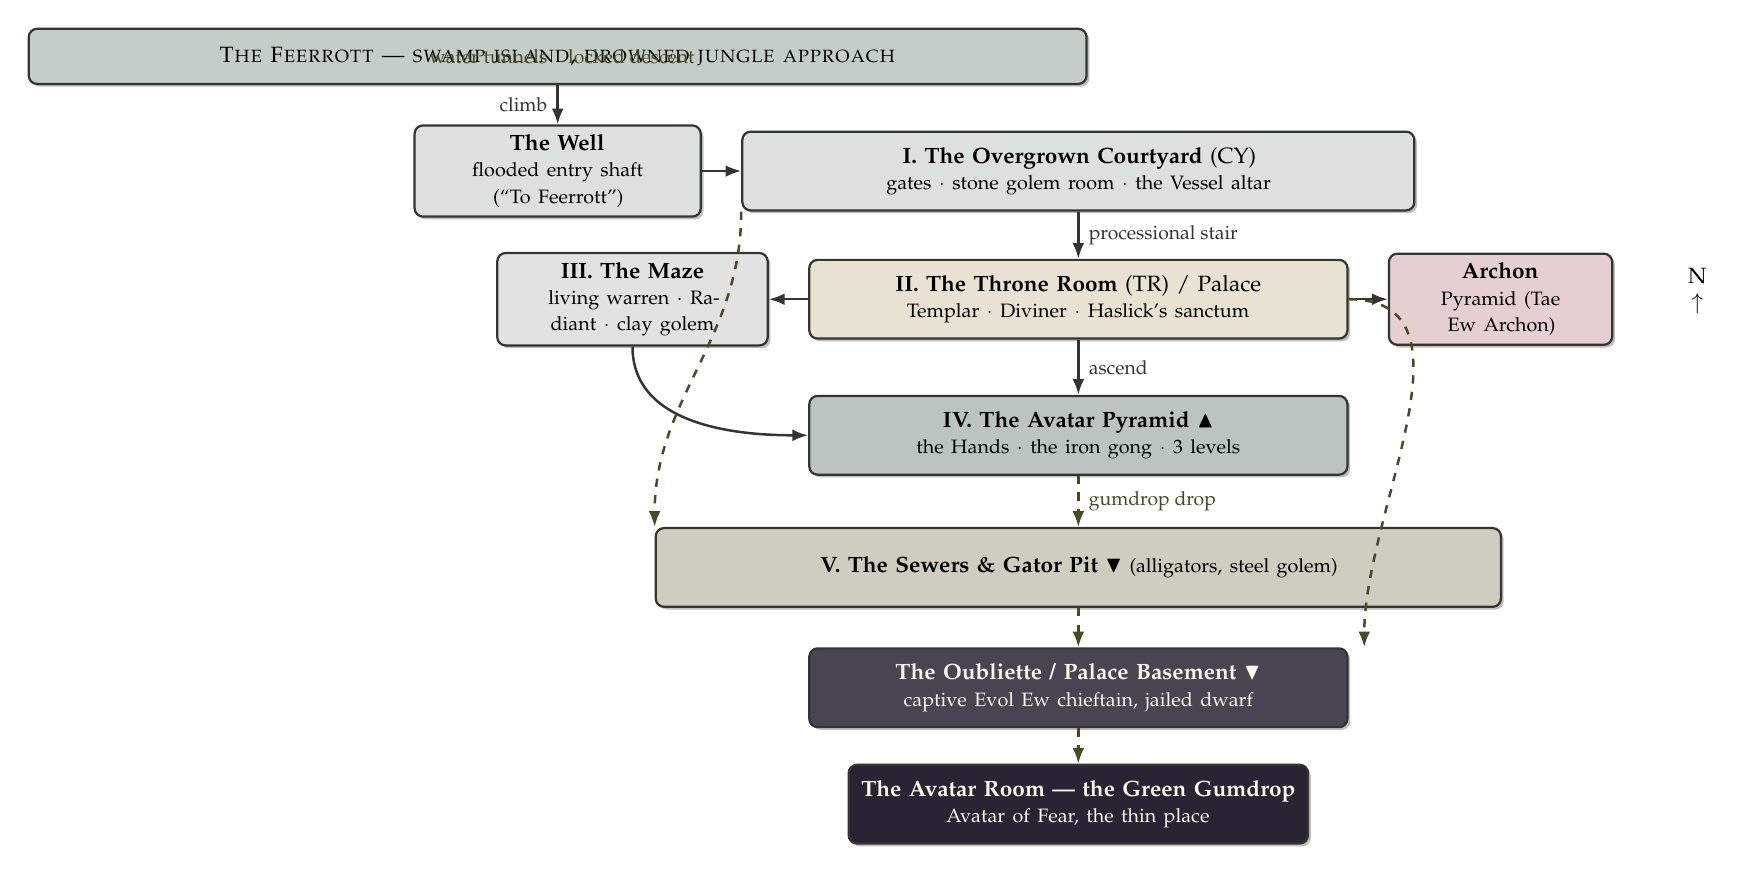
\begin{tikzpicture}[
  font=\footnotesize,
  district/.style={rounded corners=3pt, draw=stone!70!black, line width=0.8pt,
      minimum height=1.0cm, align=center, drop shadow={shadow xshift=1pt,shadow yshift=-1pt}},
  up/.style={-{Latex[length=2mm]}, line width=0.9pt, stone!70!black},
  dn/.style={-{Latex[length=2mm]}, line width=0.9pt, dashed, sewage!80!black},
]
\node[district, fill=moss!30, text width=13.2cm, minimum height=0.7cm] (jungle)
   {\scshape The Feerrott --- swamp island, drowned jungle approach};
\node[district, fill=moss!18, text width=3.4cm, below=0.5cm of jungle] (well)
   {\textbf{The Well}\\ \scriptsize flooded entry shaft (``To Feerrott'')};
\node[district, fill=moss!18, text width=8.3cm, right=0.5cm of well] (court)
   {\textbf{I. The Overgrown Courtyard} (CY)\\ \scriptsize gates $\cdot$ stone golem room $\cdot$ the Vessel altar};
\node[district, fill=gold!22, text width=6.6cm, below=0.6cm of court] (palace)
   {\textbf{II. The Throne Room} (TR) / Palace\\ \scriptsize Templar $\cdot$ Diviner $\cdot$ Haslick's sanctum};
\node[district, fill=stone!16, text width=3.2cm, left=0.5cm of palace] (maze)
   {\textbf{III. The Maze}\\\scriptsize living warren $\cdot$ Radiant $\cdot$ clay golem};
\node[district, fill=bloodred!20, text width=2.6cm, right=0.5cm of palace] (arch)
   {\textbf{Archon}\\\scriptsize Pyramid (Tae Ew Archon)};
\node[district, fill=templegreen!30, text width=6.6cm, below=0.7cm of palace] (zig)
   {\textbf{IV. The Avatar Pyramid} $\blacktriangle$\\ \scriptsize the Hands $\cdot$ the iron gong $\cdot$ 3 levels};
\node[district, fill=sewage!30, text width=10.5cm, below=0.65cm of zig] (sewer)
   {\textbf{V. The Sewers \& Gator Pit} $\blacktriangledown$ \scriptsize (alligators, steel golem)};
\node[district, fill=faceless!85, text=parch, text width=6.6cm, below=0.5cm of sewer] (base)
   {\textbf{The Oubliette / Palace Basement} $\blacktriangledown$\\ \scriptsize captive Evol Ew chieftain, jailed dwarf};
\node[district, fill=faceless, text=parch, text width=5.6cm, below=0.45cm of base] (avatar)
   {\textbf{The Avatar Room --- the Green Gumdrop}\\ \scriptsize Avatar of Fear, the thin place};

\draw[up] (jungle) -- (well) node[midway,left,font=\scriptsize]{climb};
\draw[up] (well) -- (court);
\draw[up] (court) -- (palace) node[midway,right,font=\scriptsize]{processional stair};
\draw[up] (palace) -- (maze);
\draw[up] (palace) -- (arch);
\draw[up] (palace) -- (zig) node[midway,right,font=\scriptsize]{ascend};
\draw[up] (maze) to[out=-90,in=180] (zig.west);
\draw[dn] (court.south west) to[out=-90,in=90] (sewer.north west) node[midway,left,font=\scriptsize]{water tunnels};
\draw[dn] (zig) -- (sewer) node[midway,right,font=\scriptsize]{gumdrop drop};
\draw[dn] (sewer) -- (base);
\draw[dn] (palace.east) to[out=0,in=90] ($(base.north east)+(0.2,0)$) node[midway,right,font=\scriptsize]{locked descent};
\draw[dn] (base) -- (avatar);
\node[align=center] at ($(arch)+(2.5,0.1)$) {\scshape N\\ $\uparrow$};
\end{tikzpicture}
\end{center}

\begin{center}\footnotesize
\textcolor{stone}{\scshape Legend:}\;
\tikz\node[fill=moss!25,draw=stone,rounded corners=2pt,inner sep=2pt]{}; approach/courtyard \quad
\tikz\node[fill=gold!22,draw=stone,rounded corners=2pt,inner sep=2pt]{}; throne room \quad
\tikz\node[fill=stone!16,draw=stone,rounded corners=2pt,inner sep=2pt]{}; maze \quad
\tikz\node[fill=templegreen!30,draw=stone,rounded corners=2pt,inner sep=2pt]{}; pyramids \quad
\tikz\node[fill=sewage!30,draw=stone,rounded corners=2pt,inner sep=2pt]{}; sewers \quad
\tikz\node[fill=faceless,draw=stone,rounded corners=2pt,inner sep=2pt]{}; the deep
\end{center}
\clearpage
% ============================================================ DISTRICT I
\section{District I --- The Overgrown Courtyard}

\begin{readaloud}
The jungle stops at a wall of worked stone. You climb, dripping, out of the flooded
Well that carried you up from the swamp, and the temple opens before you: a
courtyard the size of a village, half-swallowed by fig-root and vine, ringed by a
colonnade of hooded figures carved without faces. Between them, blind lizardfolk in
faded regalia move with an eerie sureness, tongues tasting the air. None of them has
eyes. All of them turn, very slightly, toward the smell of you.
\end{readaloud}

The courtyard (canonically ``CY'') is the temple's threshold and its first honest
warning. It is open to the sky, half-reclaimed by the Feerrott, and patrolled by
blind Tae Ew who navigate by scent, sound, and the taste of fear. Water-tunnels in
its floor drop straight to the Sewers and the Gator Pit below --- the fast, filthy
road to the Avatar. At its head stands the god's black-stone \textbf{Vessel},
and flanking the processional gate crouch two guardians that came through the rift:
\eqname{Fright} and \eqname{Terror}.

\begin{dmnote}[Quest Line: ``The Two Guardians'']
The inner temple opens to the bearer of an \eqname{Overseer's Sigil}, worn by the
courtyard's captain. Take one by force, theft, or ruse --- but the moment a sigil
leaves its keeper, the faceless statues shriek the alarm inward and the rift-spawned
\eqname{Fright} and \eqname{Terror} (C5) wake. A party that never trips the alarm can
instead \emph{parley} inward (C6). Because the Tae Ew are blind, disguise matters
less than \emph{scent, sound, and cadence}: moving like a pilgrim fools them where a
mask would not.
\end{dmnote}

\subsection{C1. The Well \& Broken Gate}
\begin{readaloud}
The Well is a flooded shaft ringed with frog-and-serpent carving, older and sadder
than the faceless work above; it is how the swamp-folk and the temple's own water
come and go. Beyond it, two leaning pylons frame the formal gate, their capstone
fallen into a mossy ramp. Fetishes of bone and feather hang in the gap --- and these
were not tied by blind hands.
\end{readaloud}
The entrance from the Feerrott. The fetishes are an \eqname{Evol Ew} captive-charm,
invisible to the sightless Tae Ew: a small rebellion, and a message.

\begin{techbox}
\tech{Dimensions} the Well is a 15-ft.-wide flooded shaft rising 40 ft. from the
swamp; the gate passage is 20 ft. wide, 30 ft. deep. \tech{Light} bright (open sky).
\tech{Exits} down the Well to the Feerrott; north to C2; water-grates to the Sewers
(S1). \tech{Lore} a DC 12 Survival or History check reads the Evol Ew fetish:
\emph{``the sighted have not forgotten the low door.''}
\end{techbox}

\subsection{C2. The Avenue of the Faceless}
\begin{readaloud}
Forty faceless statues line a raised avenue, twenty to a side, rain-streaked so that
each blank face seems to weep. They have no eyes to follow you --- and yet the
nearest few turn, tracking the sound of your breath and the heat of your blood.
\end{readaloud}
The idols are Cazic--Thule's alarm network. Not yet hostile, but if a sigil is
stolen or a cry raised, they relay it inward at the speed of sound, waking C5.

\begin{techbox}
\tech{Dimensions} 120 ft. long, 24 ft. wide raised avenue. \tech{Light} bright.
\tech{Exits} north to C3; branch stairs west to the Maze (District III).
\tech{Trap (idol-cry)} the first time a weapon is drawn \emph{offensively}, the
idols moan; every non--Tae Ew creature makes a DC 13 Wisdom save or is
\textbf{frightened} of the statues until the end of its next turn. This warns but
does not yet wake C5. \tech{Dread} +1 if any PC flees the avenue.
\end{techbox}

\subsection{C3. The Sacrificial Terrace \& the Vessel}
\begin{readaloud}
The avenue opens onto a terrace rising to a broad, shallow bowl of black stone: the
Vessel. Wide is its brim, worn smooth and stained not red but \emph{black}, layer on
layer, older than any red could stay. Two of its handles have been snapped off ---
long ago, and never repaired, as though the wound were now part of the rite. A
gutter runs from its lip toward a drain that mutters somewhere below.
\end{readaloud}
The heart of the temple's economy of fear. The \eqname{Vessel} is where captives are
bled; the Rallosians defiled it in the long-ago (hence the broken handles), and the
Tae Ew have used it, defiled, ever since. If the party lingers, they may witness a
sacrifice --- a chance to intervene, and to raise Dread if they do not.

\begin{itemize}
\item An \textbf{Overseer} (a \textbf{Tae Ew Temple Guard}, App.\ A) presides,
bearing the courtyard's one \eqname{Overseer's Sigil}. Blind; baitable; pickpocketable
(DC 15 while distracted by sound).
\item A work-gang of three \textbf{Alliz Evol Ew Captives} (App.\ A) hauls silt,
hobbled and watched. A freed captive becomes a temporary ally and points the party
toward the Oubliette and their chieftain (District V).
\item The gutter-drain descends to the Sewers (S3, the Bloodstream); the water-tunnel
at the terrace edge drops to the Gator Pit (S-district).
\end{itemize}

\begin{techbox}
\tech{Dimensions} 40 ft. by 40 ft., three 2-ft. tiers; the Vessel is 8 ft. across.
\tech{Light} bright. \tech{Exits} north to C4 (stone golem room) and the Processional
Stair (C7); drains down to the Sewers/Gator Pit. \tech{Feature} DC 14 Religion reads
the Vessel's cycle: the next great rite is due \emph{soon} (ties to District IV).
\end{techbox}

\subsection{C4. The Stone Golem Room}
\begin{readaloud}
A raised chamber off the terrace, its floor a mosaic of the temple's history worn to
ghosts underfoot. At its center stands what you first take for another faceless
statue --- until it turns its head, grinding, and steps down off its plinth.
\end{readaloud}
Canonically the ``Stone'' camp. A \textbf{Stone Golem} (App.\ A) guards the way up,
and the priesthood can raise more of its kind. A dangerous chokepoint: noise here
draws Tae Ew from the Throne Room above.

\begin{techbox}
\tech{Dimensions} 40 ft. by 30 ft., raised 5 ft. above C3. \tech{Light} dim.
\tech{Exits} up to the Processional Stair (C7) and the Throne Room (District II);
tunnels to the middle and top levels of the Avatar Pyramid (District IV).
\tech{Warning} pulling a fight out of this room drops lizards through the ceiling
into the Throne Room below --- who return with friends.
\end{techbox}

\subsection{C5. Fright \& Terror, the Rift-Guardians}
\begin{readaloud}
Two squat watch-plinths flank the head of the terrace. Atop the left crouches a
thing all jaws and no eyes; atop the right, a thing all eyes and no jaws. They are
not stone. They are the color of the dark between torches, and they came from
somewhere the world was never meant to touch. When the alarm comes, they uncoil.
\end{readaloud}
\eqname{Fright} and \eqname{Terror} (App.\ A, \CR{6} each) are planar fear-elementals
that slipped through the rift and were bound to the gate. Dormant until an alarm, they
animate together and amplify each other's terror. This is the district's boss fight
and the price of the front door.

\begin{dmnote}[Fighting the Twins]
While both live, each has advantage on saves and its fear-aura DC rises by 2. Killing
one first collapses the buff --- reward players who see it. If the alarm was never
tripped, the twins never wake, and a stealthy party simply passes two very unsettling
shapes. Let that be a real reward.
\end{dmnote}

\begin{techbox}
\tech{Dimensions} each plinth 15 ft. square, 10 ft. tall. \tech{Light} bright.
\tech{Exits} between them stands the foot of the Processional Stair (C7).
\tech{Trigger} the idol-network alarm (C2) or a stolen sigil borne within reach.
\end{techbox}

\subsection{C6. The Overseer's Post}
\begin{readaloud}
A lean-to of salvaged temple stone shelters a brazier, a rack of notched
tally-sticks, and a hammock of processional banners. Whoever draws the short watch
lives here: blind, bored, and desperate for anything to break the sameness of the
days.
\end{readaloud}
The social heart of the courtyard. The guard here can be bribed, cowed, deceived, or
--- if the party moves and sounds like returning pilgrims --- \emph{escorted inward}
with a borrowed sigil, bypassing C5. The Tae Ew respect rank and ritual cadence; sound
the part and they will not smell the lie.

\begin{techbox}
\tech{Dimensions} 15 ft. by 15 ft. \tech{Light} firelit. \tech{Exits} adjacent to
C5/C7. \tech{Social} Deception/Persuasion DC 13 to pass as pilgrims (advantage if the
party carries a temple relic or intones a rite-phrase learned in C3 or the
Scriptorium, P6); Intimidation DC 16. \tech{Reward} success yields a loaned sigil and
safe passage --- until an obvious blasphemy.
\end{techbox}

\subsection{C7. The Processional Stair}
\begin{readaloud}
A grand stair climbs from the terrace toward green-bronze doors above. Each step is
carved with a single word in the old backward tongue; sounded out in sequence as you
climb, they spell a sentence you will wish you had not understood.
\end{readaloud}
The formal route from Courtyard up to the Throne Room. The doors require an
\eqname{Overseer's Sigil}.

\begin{techbox}
\tech{Dimensions} 60 steps over 30 ft. of rise. \tech{Light} bright below, dim above.
\tech{Exits} up to the Throne Room (P1); doors sealed (AC 17, 60 HP, DC 20 Strength
to force, which trips the C2 alarm). \tech{Lore} DC 12 History (or anyone who reads
the tongue backward) translates the litany, promising the reader to the Faceless;
reading it aloud grants advantage on the pilgrim ruse in C6.
\end{techbox}

\subsection{C8. The Water Tunnels}
\begin{readaloud}
Behind a curtain of root, two flooded throats descend into the dark, breathing up
cold and rot. One drops toward the mutter of running water; the other toward a
deeper, wetter sound, and the slow slap of something large turning over in a pool.
\end{readaloud}
The courtyard's back doors: one water-tunnel drops to the \textbf{Sewers} (S1), the
other to the \textbf{Gator Pit}. A party willing to arrive at the temple's flooded
bottom first can run the whole dungeon inside out.

\begin{techbox}
\tech{Dimensions} two 4-ft. flooded chutes dropping 40 ft. \tech{Light} none.
\tech{Exits} down to the Sewers (S1) and the Gator Pit (S-district). \tech{Hazard}
DC 13 Athletics/Acrobatics per 20 ft.; failure is a slide (2d6 bludgeoning) and a
loud, prone arrival --- in the Gator Pit, directly among alligators.
\end{techbox}
% ============================================================ DISTRICT II
\clearpage
\section{District II --- The Throne Room \& Palace}

\begin{readaloud}
Beyond the bronze doors the temple remembers what it used to be. The rot falls away;
the floors are swept, the braziers lit, the air thick with incense over an
under-smell of reptile musk and old meat. Blind servitors in threadbare finery bow
as you pass, tasting the air, mistaking you --- for now --- for someone who belongs.
This is a court that has performed its own importance to a watching god for an age,
and it will eat you before it admits the empire is gone.
\end{readaloud}

The Throne Room (canonically ``TR'') and its surrounding halls are the seat of the
Cazicite priesthood. It is inhabited, orderly, and lethal to the socially clumsy: a
drawn blade in the wrong hall brings the whole priesthood down at once, and they
\emph{heal each other through the walls}. The party's goals here are the patriarch
\eqname{Tool Haslick} (P8), the Reliquary (P5), and the key to the locked descent
(P10).

\begin{dmnote}[Quest Line: ``The First Cannibal'']
Haslick means to complete the \eqname{Great Rite}: to wake the Avatar fully and ride
its return to power. He needs the sacred \eqname{Hands} attended (District IV), a
worthy sacrifice (the captive Evol Ew chieftain, District V), and the litany from the
Scriptorium (P6). The party can \textbf{stop} the rite --- kill Haslick, free the
chieftain, or interrupt the ritual at the pyramid --- or \emph{let it proceed} and
face a fully-woken Watcher. Haslick carries the \eqname{Basement Key} (P10) and the
\eqname{Lizardskin Tribal Mask} (App.\ B).
\end{dmnote}

\subsection{P1. The Hall of Bowed Heads}
\begin{readaloud}
A gallery of kneeling statues bowed so low their faceless heads nearly touch the
floor, forming an arcade you must stoop to pass. The message needs no eyes to read:
here, you are lower than the lowest of them.
\end{readaloud}
The receiving hall. Blind servitors (noncombatant \textbf{commoners}) expect ritual
deference sounded aloud; belligerence summons guards.

\begin{techbox}
\tech{Dimensions} 80 ft. by 20 ft.; ceiling 6 ft. beneath the bowed heads (Medium
creatures move at half speed unless they crawl). \tech{Light} dim. \tech{Exits} south
to C7; north to the Throne (P4); side doors to P5 (reliquary), P6 (scriptorium),
P7 (baths). \tech{Social} a failed deference check (DC 12) marks the party as suspect.
\end{techbox}

\subsection{P2. The Diviner's Antechamber}
\begin{readaloud}
A waiting room for supplicants, if the supplicants were meant to leave shaking. The
\eqname{Tae Ew Diviner} holds court here among a haze of enchantment, her blind head
cocked, sorting truth from lie by the flutter of your pulse.
\end{readaloud}
The \textbf{Tae Ew Diviner} (App.\ A, canonical enchanter, drops the
\eqname{Lizardscale Mantle}) screens visitors and is the party's best
intelligence source --- if flattered or deceived --- on the rite's timing and the
Hands.

\begin{techbox}
\tech{Dimensions} 30 ft. by 30 ft. \tech{Light} dim. \tech{Exits} to P1, P4.
\tech{Hazard} the Diviner's charm magic; a party that fights here risks being turned
on one another (she favors \textit{hold person} and confusion effects).
\end{techbox}

\subsection{P3. The Royal Gallery}
\begin{readaloud}
Formal reliefs of the Tae Ew line, every royal face chiseled deliberately blank in
the same rite that blinded them. Only regalia tells one dead patriarch from the
next. At the gallery's end, one relief has been re-carved fresh --- and it shows a
figure crowning himself with a crown you have not seen worn.
\end{readaloud}
Lore and foreshadowing: the fresh relief shows \eqname{Haslick} crowning himself, the
first cannibal reaching for kingship as well as prophecy. An Evol Ew captive, if
present, recognizes the crown as spoil taken from their own chieftain.

\begin{techbox}
\tech{Dimensions} 60 ft. by 15 ft. \tech{Light} dim. \tech{Exits} loops P1 to P4.
\tech{Lore} DC 12 History reconstructs the dynasty and the Green Dawn; DC 15 reveals
the Avatar was never destroyed, only re-buried --- and is woken by the gong.
\end{techbox}

\subsection{P4. The Whispering Court}
\begin{readaloud}
The throne room proper. A dais of black glass supports a throne carved as a single
screaming, faceless head, its open mouth the seat. Upon it sits the
\eqname{Tae Ew Templar}, blind and serene, and the air is full of whispering, as
though the whole dead court still convenes here and has only just stopped talking to
taste you.
\end{readaloud}
The ceremonial center. The \textbf{Tae Ew Templar} (App.\ A, canonical cleric on the
throne, drops the \eqname{Lizardscale Cloak}) presides, flanked by guards; the
whispering is a standing minor fear effect. The Templar heals every Tae Ew in
earshot --- through the walls.

\begin{techbox}
\tech{Dimensions} 50 ft. by 50 ft., dais 3 ft. high. \tech{Light} dim, braziers.
\tech{Exits} to P2, P3, P8 (Haslick's sanctum, behind the throne), P10 (locked
descent). \tech{Aura} a creature ending its turn on the dais makes a DC 12 Wisdom
save or hears the whispers name its worst fear; at Dread 4+ it is \textbf{frightened}
1 round.
\end{techbox}

\subsection{P5. The Reliquary}
\begin{readaloud}
A vault of the empire's holy loot: green-bronze reliquaries, weapons furred with
verdigris, scale-armor folded in cedar. One shelf has been dusted and left
conspicuously empty, awaiting something not yet returned.
\end{readaloud}
The treasure room, locked (DC 17 thieves' tools; key on the P2 Diviner or Haslick).
Contains a curated hoard (App.\ B): the \eqname{Rubicite Breastplate}, the
\eqname{Ravenscale Chestguard}, a \eqname{Lizardscale Belt}, and a \eqname{Lizard
Blood Potion}. The empty shelf awaits the \eqname{Idol of Thule}, taken up to the
pyramid for the rite.

\begin{techbox}
\tech{Dimensions} 25 ft. by 20 ft. \tech{Light} none. \tech{Exits} single door to P1.
\tech{Trap} opening a case without speaking the litany (P6) triggers a \emph{glyph of
fear}: 20-ft. radius, DC 15 Wisdom or frightened 1 minute, and the alarm reaches
Haslick.
\end{techbox}

\subsection{P6. The Scriptorium}
\begin{readaloud}
Shelves of clay tablets and skin scrolls, tended by an ancient priest who reads with
his fingertips --- as all of them now must. The knowledge of the whole god-city is
here: its rites, its wards, its history, and the litany that unlocks every holy
thing in the Palace.
\end{readaloud}
The information hub. The blind archivist (a noncombatant priest who will scream for
guards but not fight) can be persuaded, deceived, or robbed. Reading here grants the
\emph{litany} (defuses P5), the form of the \emph{Great Rite} (District IV), the
location of the captive chieftain (District V), and --- on a second DC 15 check ---
the Avatar's weakness: it can be \textbf{banished} by an unfrightened creature holding
the Idol of Thule.

\begin{techbox}
\tech{Dimensions} 40 ft. by 30 ft. \tech{Light} dim. \tech{Exits} to P1.
\tech{Research} 30 minutes and DC 13 Investigation for the litany; DC 15 for the
banishing weakness and the truth of the gong.
\end{techbox}

\subsection{P7. The Priest-Kings' Baths}
\begin{readaloud}
Steaming tiled pools, a decadence the priests still insist upon. Off-duty clergy soak
here, unarmored and blind and unguarded, trading gossip that would get them flayed if
the wrong ear heard it.
\end{readaloud}
A rare soft target and a superb infiltration point: priests here are unarmored (AC 10)
and full of information. Strike here to thin the priesthood before P8, or simply
listen.

\begin{techbox}
\tech{Dimensions} 40 ft. by 25 ft., pools 4 ft. deep. \tech{Light} steamy, dim
(lightly obscured --- which does not hinder the blind). \tech{Exits} to P1 and a
servants' passage into the Maze (District III). \tech{Occupants} 1d3 unarmored
priests (use \textbf{Tae Ew Diviner} or guard stats, unarmored).
\end{techbox}

\subsection{P8. Haslick's Sanctum}
\begin{readaloud}
Behind the screaming throne, a private chapel no larger than a bedchamber, its walls
papered in flayed faces. At its center stands something that was the first of its
kind and has refused, for an age, to finish dying: a withered lizard-patriarch, his
own face long since ritually erased, his jaws still wet. When he speaks, the voice
comes from every flayed face on the walls at once. ``You are late,'' says Tool
Haslick, the First Cannibal. ``The god has been expecting you.''
\end{readaloud}
\eqname{Tool Haslick} (App.\ A, \CR{9}) is the district boss: the tribe's founding
patriarch, sustained past death by the necromancy he pioneered, architect of the
coming apocalypse. He fights with fear magic, the flayed-face walls, and summoned
undead. He carries the \eqname{Basement Key}, the \eqname{Lizardskin Tribal Mask}
(App.\ B), and knows the party's names before they speak.

\begin{dmnote}[Haslick's Gambit]
Haslick would rather the party \emph{help} him: he offers them the chieftain's
sacrifice and a share of the god's favor. A depleted party might take the deal ---
and run the pyramid climax as accomplices. His death drops the Basement Key. Below
20 HP he may crumble to ash and re-form at the pyramid to officiate the rite in
person.
\end{dmnote}

\begin{techbox}
\tech{Dimensions} 20 ft. by 20 ft. \tech{Light} dim, guttering. \tech{Exits} to P4.
\tech{Feature} the flayed-face walls let Haslick ``speak'' from any face once per
turn, imposing disadvantage on a chosen creature's first save that round against his
magic.
\end{techbox}

\subsection{P9. The Royal Larder}
\begin{readaloud}
The kitchens: fire-pits, hanging carcasses of swamp beasts --- and, in a corner
cage, a huddle of captured Evol Ew hatchlings, sighted and terrified, being fattened
for the Vessel. A cook the size of a door turns toward the sound of you with a
cleaver in each hand.
\end{readaloud}
A moral pressure-point. Freeing the hatchlings (a \textbf{Tae Ew Broodmother} guards
them, App.\ A) lowers Dread by 2 and earns deep Evol Ew loyalty in District V.

\begin{techbox}
\tech{Dimensions} 40 ft. by 30 ft. \tech{Light} firelit. \tech{Exits} to P1 and a
greasy chute down to the Sewers (S2). \tech{Occupants} 1 Broodmother, 2 Evol Ew
hatchlings (noncombatant). \tech{Dread} -2 if the hatchlings are freed and escorted
to the captives below.
\end{techbox}

\subsection{P10. The Locked Descent}
\begin{readaloud}
A stair spirals down from a door of black iron whose lock is a single faceless mouth
waiting to be fed a key. Warm air is drawn steadily downward, as though something far
below is breathing in.
\end{readaloud}
The ``royal'' route to the basement and the pit, as opposed to the captives' flooded
tunnels. Requires the \eqname{Basement Key} from Haslick.

\begin{techbox}
\tech{Dimensions} spiral stair descending 50 ft. \tech{Light} none. \tech{Exits} down
to the Oubliette / Palace Basement (S5). \tech{Lock} AC 19, 80 HP, immune to
nonmagical damage; the Basement Key or DC 22 thieves' tools opens it. Forcing it
magically alerts all of District V.
\end{techbox}
% ============================================================ DISTRICT III
\clearpage
\section{District III --- The Maze of Ten Thousand Doors}

\begin{readaloud}
This is where the god-city actually lives. Not a dungeon --- a warren. Narrow lanes
wind between stacked stone dwellings, doorways hung with beaded curtains, cook-smoke
curling up through light-shafts to no purpose, for no one here has eyes to want the
light. Blind hatchlings chase a beetle by sound and freeze when they hear you. A
lullaby is being clicked and hissed somewhere close. The Maze does not want to fight
you. It wants you gone before you frighten the brood --- and before anyone gets
hungry.
\end{readaloud}

The Maze is the residential warren of the common Tae Ew --- everyone who is neither
priest nor patriarch. It is deliberately labyrinthine (outsiders get lost; residents
never do, moving by memory and scent) and it is \emph{full of people}: warders, pages,
broodlings, elders, hatchlings, all blind, all willing to eat the weak. It connects
the Courtyard to the Pyramid, and it holds a \eqname{Wizard Pyramid} spire that
mages use to teleport straight in.

\begin{dmnote}[Quest Line: ``Ten Thousand Doors'']
Two threads. First, \textbf{navigation}: cross the Maze without a map using the
getting-lost system below, unless the party earns a guide. Second, the
\textbf{captives}: freeing the Evol Ew held here and in the Oubliette gives the party
a warband --- but the Evol Ew fight \emph{for their chieftain first} and will turn on a
party that uses and abandons them. A guide (a freed Evol Ew, a bribed elder, or the
P9 hatchlings' gratitude) removes the getting-lost penalty entirely.
\end{dmnote}

\begin{dmnote}[The Getting-Lost System]
Moving between the lettered locales below without a guide, roll a d6 each transition:
on 1--2 the party arrives at a random adjacent locale (roll below) and 1d4 turns
pass. A DC 14 Wisdom (Survival) or Intelligence (Investigation) check --- marking
walls, following smoke or water --- converts a failure to a success. With a guide, no
roll. Random locale (d6): 1: M1, 2: M2, 3: M3, 4: M4, 5: M5, 6: M6.
\end{dmnote}

\subsection{M1. The Threshold Warren}
\begin{readaloud}
The Maze's edge, where the swept order of the Palace frays into lived-in clutter.
Dyed cloth crosses overhead; an old matron sits shelling swamp-nuts by feel and turns
her eyeless face toward you with a wary, ancient patience.
\end{readaloud}
The buffer between Palace and warren, and the best place to make contact. The matron
(a noncombatant elder) will, for courtesy or a gift, offer a warning, a rumor, or ---
rarely --- a grandchild as a guide.

\begin{techbox}
\tech{Dimensions} a knot of 5-ft. lanes over roughly 60 ft. square. \tech{Light} dim.
\tech{Exits} to the Palace (P1/P7) and deeper into M2--M6. \tech{Social} moving as
guests (no weapons drawn, quiet cadence) grants advantage on Maze social checks; a
single act of violence sets the whole district hostile.
\end{techbox}

\subsection{M2. The Broodmother's Nursery}
\begin{readaloud}
A warm, humid chamber of sand-beds where clutches of leathery eggs incubate under
glowing fungus. Broodmothers move among them, turning eggs by touch, crooning. It is
a place of tenderness --- which makes it the most dangerous room in the Maze, for
there is nothing these blind guardians will not do.
\end{readaloud}
Two \textbf{Tae Ew Broodmothers} (App.\ A) defend it with berserk ferocity if
threatened, but ignore a respectful party. A moral fulcrum.

\begin{techbox}
\tech{Dimensions} 40 ft. by 30 ft. \tech{Light} fungal (irrelevant to the blind).
\tech{Exits} to M1, M3. \tech{Dread} +2 if the nursery is attacked; the district
mobilizes.
\end{techbox}

\subsection{M3. The Commons \& Cooking Pits}
\begin{readaloud}
The widest space in the warren: communal cook-fires, drying racks, a cistern, and a
crowd. Dozens of blind lizardfolk pause mid-meal --- and you do not care to look too
closely at the meal --- and turn as one toward the sound of strangers. For one held
breath, the whole city could go either way.
\end{readaloud}
The social climax of the Maze. Negotiate passage openly (DC 15, modified by prior
conduct) and the commons will look the other way, even hide the party from patrols.

\begin{techbox}
\tech{Dimensions} 60 ft. by 50 ft. \tech{Light} firelit. \tech{Exits} all directions
(M1--M6, and a lane to the Pyramid, District IV). \tech{Occupants} 2d6 commoners,
2 \textbf{Tae Ew Temple Guards}. \tech{Social} a won-over crowd grants a guide and
advantage on the Pyramid approach.
\end{techbox}

\subsection{M4. The Captive Pens}
\begin{readaloud}
The lanes turn cruel. Cage-doors of green bronze line a sunken row, and behind them
crowd the captives: gaunt Evol Ew with their sight intact and staring, a jailed
dwarf in rusted mail cursing steadily under his breath, a huddle of gnomish mages
whispering half-remembered spells. A single overseer paces the row, bored, tapping a
goad against the bars.
\end{readaloud}
The engine of the ally-warband. Captured \textbf{Alliz Evol Ew} (App.\ A) crowd the
pens under a light guard, alongside a canonical \textbf{jailed dwarven mercenary} and
a cage of gnomish mages. Freeing them is loud and consequential: a running battle
through the Maze, and a warband --- though the Evol Ew fight for their chieftain first.

\begin{dmnote}[Running the Uprising]
Track a morale clock: captives start at Morale 3. Each freed pen, each downed
overseer, and each hatchling returned (from P9) adds 1; each captive death subtracts 1.
At Morale 5+, the freed captives hold the Maze on their own; at 0 they scatter. Freeing
the chieftain (District V) sets Morale to maximum and turns the warband into an army
for the finale. The jailed dwarf, if freed, fights as a \textbf{veteran} and is worth a
laugh and a debt.
\end{dmnote}

\begin{techbox}
\tech{Dimensions} 50 ft. sunken row, cages 8 ft. deep. \tech{Light} dim.
\tech{Exits} to M3, M5, and a service tunnel to the Sewers (S2). \tech{Lock} AC 15,
DC 13 thieves' tools, or the overseer's key. \tech{Dread} -1 per pen freed.
\end{techbox}

\subsection{M5. The Fungal Middens}
\begin{readaloud}
Where the Maze meets the wet: a low, dripping hall where the city's waste composts
into the glowing fungus that lights homes no one can see. The floor is soft with
centuries of rot, and something down here has been eating the fungus and growing fat.
\end{readaloud}
The Maze's rot-line and its bleed into the Sewers. A \textbf{Fungal Horror}
(App.\ A) lairs here, tolerated as a household pest; a stealth route down to
District V that avoids the locked descent.

\begin{techbox}
\tech{Dimensions} 40 ft. by 40 ft., ceiling 6 ft. \tech{Light} fungal (dim).
\tech{Exits} to M2/M4 and down to the Sewers (S2). \tech{Hazard} spore clouds: a
creature that takes damage here makes a DC 12 Con save or is poisoned 1 minute.
\tech{Terrain} the whole floor is difficult terrain.
\end{techbox}

\subsection{M6. The Wizard Spire \& the Clay Golem}
\begin{readaloud}
A dead-end court dominated by a slender spire of green stone, its tip humming with
bound arcane force --- the point to which the temple's mages teleport, and past which
a thing of wet grey clay endlessly patrols, molded in the shape of a faceless man.
\end{readaloud}
Canonically the \eqname{Wizard Pyramid} (a teleport-in point) and the roaming
\textbf{Clay Golem} (App.\ A) that guards it, wandering as far as the portal before
returning. \eqname{Radiant}, a Tae Ew rogue traitor-for-hire (App.\ A), also stalks
the Maze near here.

\begin{techbox}
\tech{Dimensions} 25 ft. dead-end court, spire 30 ft. \tech{Light} arcane glow.
\tech{Exits} to M3. \tech{Feature} the spire is a live teleport anchor; a caster who
studies it (DC 15 Arcana) can later use it as a \textit{teleport}/\textit{word of
recall} destination. \tech{Roamer} the Clay Golem patrols on a circuit; time it.
\end{techbox}
% ============================================================ DISTRICT IV
\clearpage
\section{District IV --- The Avatar Pyramid}

\begin{readaloud}
It dwarfs everything. From the warren's lanes you had no sense of it, but here it
climbs step over blood-black step into the dark of the cavern-roof, and at its
summit two enormous carved \emph{hands} rise from the stone --- severed clean at the
wrists, palms open, fingers reaching, as though the god were pushing up out of the
world from below. A procession of blind priests winds up the pyramid's face, bearing
between them something that struggles and weeps. The whole god-city is oriented
toward this. The pyramid is not \emph{in} the temple. The pyramid is why the temple
exists.
\end{readaloud}

The Avatar Pyramid is the ritual heart of the god-city and the one place the party
climbs \emph{upward} before the final plunge. Canonically it has three levels: a
\textbf{top} crawling with the temple's deadliest lizards and silvered guards; a
water-filled \textbf{middle}; and, at the \textbf{bottom}, the green ``gumdrop'' that
holds the Avatar of Fear (the finale, District V). You can fall between the levels.
Here Haslick's Great Rite comes to a head --- and here stands the iron gong that wakes
the Watcher.

\begin{dmnote}[Quest Line: ``The Ascension Interrupted'']
The Great Rite needs the \eqname{Idol of Thule} (attended at the Hands) and a worthy
sacrifice (the Evol Ew chieftain, dragged up from below). The party may: (a)
\textbf{seize the Idol} --- the one thing that can banish the Avatar peacefully; (b)
\textbf{interrupt the rite} at the Hands, fighting Haslick and his priests; or (c)
\textbf{let it complete}. Two clocks live here: the rite, and the \textbf{iron gong}
--- for whoever strikes the gong wakes the Sleeping Watcher, whether they mean to or
not. \eqname{Dread}, the rift-wraith (App.\ A), guards the Hands.
\end{dmnote}

\subsection{Z1. The Base Ambulatory}
\begin{readaloud}
A colonnaded walk rings the pyramid's foot, its inner wall one continuous relief that
tells the whole terrible history in carved panels: the raising of the city, the
blessing and the rift, the broken oath, the Green Dawn falling green upon the ogres.
The final panels are blank. They are waiting to be carved.
\end{readaloud}
The narrative payoff: the reliefs confirm the full lore, and the blank panels make
plain that Haslick means to write the next chapter tonight.

\begin{techbox}
\tech{Dimensions} a 15-ft. walk ringing a 100-ft.-square base. \tech{Light} dim,
green flame-glow from above. \tech{Exits} to the Maze (M3) and Courtyard (C4); four
stairs ascend the faces to Z2; tunnels from the Stone Golem room (C4) enter the top
and middle levels. \tech{Lore} DC 12 History reads the reliefs; DC 15 confirms the
Avatar is banished, not slain, by the Idol of Thule.
\end{techbox}

\subsection{Z2. The Top Level --- Silvered Ranks}
\begin{readaloud}
The upper terraces belong to the temple's elite: silvered guards pacing the ledges,
a crusader in decayed black mail buffing his blind kin, obelisks at the four corners
catching the green light. The drop yawns at the terrace edge, and gators churn in the
flooded pits far below.
\end{readaloud}
The deadliest camp: \textbf{Silvered Guards} and a \textbf{Lizard Crusader}
(shadowknight; use \textbf{Tae Ew Temple Guard} with the crusader note in App.\ A).
Nearby, on a bridge in the neighboring \eqname{Archon Pyramid}, the \textbf{Tae Ew
Archon} (App.\ A, wizard) drops the \eqname{Lizardscale Belt} and the
\eqname{Ravenscale Armguards}.

\begin{techbox}
\tech{Dimensions} 12-ft. terraces around the pyramid; corner obelisks 15 ft.
\tech{Light} dim. \tech{Exits} tunnels to C4; down to Z3; the Archon's bridge lies
across a gap (levitation or a DC 16 climb). \tech{Hazard} knock-back effects and
terrace edges: a creature knocked off falls to the water level (Z3) or the Gator Pit.
\end{techbox}

\subsection{Z3. The Middle Level --- The Drowned Tier}
\begin{readaloud}
The pyramid's middle is flooded: a black interior lake beneath a low ceiling, pillars
rising from the water, the surface breathing mist. Things move under it, unhurried.
The only dry footing is a rim of ledges, and the water pulls, faintly, toward a sluice
that mutters downward into green light.
\end{readaloud}
The water-filled middle tier, a transition between the elite top and the Hands
chamber. Alligators lair here; the sluice drains toward the gumdrop below.

\begin{techbox}
\tech{Dimensions} a 60-ft. flooded interior, water 8 ft. deep. \tech{Light} dim,
greenish. \tech{Exits} up to Z2; a concealed hatch (DC 15 Perception) to the Hands
chamber (Z4); the sluice drops to the Avatar Room (District V). \tech{Hazard} 1d2
\textbf{Alligators} (App.\ A); swimming in armor is a DC 12 Athletics check.
\end{techbox}

\subsection{Z4. The Chamber of the Hands}
\begin{readaloud}
Within the pyramid's hollow heart rise the Hands: two colossal fists of black jade,
severed at the wrist, thirty feet of reaching stone, palms cupped as if to catch what
falls. Between them stands a squat idol of the same jade with a smooth blank oval
where a face should be --- the Idol of Thule --- humming with a cold that has weight.
An iron gong, cracked and ancient, hangs to one side. And something is coiled in the
green dark between the Hands: it uncoils to regard you with the certainty of a
nightmare that already knows it is yours.
\end{readaloud}
The set-piece. Why only hands? Because the god walked among the Tae Ew and made them
carve his likeness --- but each time he left, they stopped, and each time he returned,
they began again \emph{at the wrist}; and so the wrists are all that were ever
finished. \eqname{Dread}, the rift-wraith (App.\ A, \CR{8}), guards the Hands, the
\eqname{Idol of Thule} (App.\ B), and the cracked \textbf{iron gong} --- the same
gong Vashahkti shattered to wake the Watcher in the long-ago.

\begin{dmnote}[The Idol, and the Gong]
The \eqname{Idol of Thule} is the campaign's keystone: an unfrightened bearer can use
it to \emph{banish} the Avatar rather than grind through its full stat block. The
\textbf{iron gong} is the wildcard: striking it (deliberately, or by a stray blast in
the fight with Dread) instantly wakes the Avatar and begins the finale --- possibly
before the party is ready. Telegraph both clearly; let the players choose whether to
seize the Idol before anyone touches the gong.
\end{dmnote}

\begin{techbox}
\tech{Dimensions} 60 ft. square, 90 ft. tall (the Hands fill the vault). \tech{Light}
green flame. \tech{Exits} down the sluice/shaft to the Avatar Room (District V);
up to Z3. \tech{Aura} constant fear pressure: a creature starting its turn here makes
a DC 13 Wisdom save or has disadvantage on attacks that turn; Dread is immune and
regains 5 HP per failure. \tech{Gong} AC 10; any thunder/force damage or a struck
blow rings it --- see the finale (S8).
\end{techbox}
% ============================================================ DISTRICT V
\clearpage
\section{District V --- The Sewers \& the Green Gumdrop}

\begin{readaloud}
Below everything, the god-city drowns. The Sewers are its gut and its graveyard:
flooded channels running with the runoff of a thousand rites, the water thick with
blood gone to rot and loud with the slap of alligators. Here the temple stops
pretending to be a place of worship and admits what it is --- a machine for making
fear, with a drain at the bottom that opens onto the mouth of a god.
\end{readaloud}

District V is the temple's foundation and its terminus: the flooded \textbf{Sewers},
the \textbf{Gator Pit} (canonically ``Alligator Alley''), the \textbf{Oubliette}
where the Evol Ew chieftain is caged, and the green \textbf{gumdrop} that holds the
\eqname{Avatar of Fear}. It can be entered from the top (the pyramid's sluice, the
P10 descent, the M5 middens) or from the bottom (the courtyard water-tunnels) --- run
the latter and the party takes the whole adventure inside out.

\begin{dmnote}[Quest Line: ``The Pit of Fear'' --- the Finale]
Everything converges. The party's approach sets the difficulty:
\begin{itemize}
\item \textbf{With the Idol of Thule} and an \emph{unfrightened} bearer, the Avatar is
\textbf{banished} in three rounds of channeling rather than fought to 0 HP.
\item \textbf{With the chieftain freed} (S5) and a high captive Morale, an Evol Ew
warband floods in and roughly halves the Avatar's effective threat.
\item \textbf{With neither}, the party fights the full Avatar of Fear (App.\ A) head-on
--- brutal, and enriched by its \emph{harm touch}.
\item If \textbf{the gong was struck} or \textbf{the Rite completed}, the Avatar is
already awake and waiting, and Haslick attends as its herald.
\end{itemize}
\end{dmnote}

\subsection{S1. The Drowned Undercroft}
\begin{readaloud}
The courtyard water-tunnel spits you chest-deep into a flooded hall of sunken
pillars, the waterline mapped in sick green slime. Something long and pale glides
between the columns, unhurried, and does not surface.
\end{readaloud}
The bottom-entry landing (from C8). A drowned introduction to the Sewers, patrolled by
alligators and the occasional blind lizard scout.

\begin{techbox}
\tech{Dimensions} 60 ft. by 40 ft., water 4--5 ft. deep. \tech{Light} dim (slime).
\tech{Exits} up the tunnel to C8; on to S2/S3. \tech{Hazard} 1 \textbf{Alligator}
(App.\ A); deep pockets (DC 12 Perception) drop creatures into 15-ft. sink-holes.
\end{techbox}

\subsection{S2. The Weeping Cisterns}
\begin{readaloud}
A junction of great cisterns where every chute and drain in the temple empties. Blind
lizards work the sluice-gates by touch; captive Evol Ew voices echo from the
pipe-mouths, and sighted eyes shine from the dark, deciding whether you are prey,
predator, or the answer to an old prayer.
\end{readaloud}
The Sewers' hub and the free captives' listening-post. First contact with Evol Ew who
have escaped into the low country: if the party has freed captives above, they reveal
themselves as allies; if not, they shadow the party warily.

\begin{techbox}
\tech{Dimensions} a 50-ft. octagonal junction over 6-ft.-deep water. \tech{Light} dim.
\tech{Exits} chutes up to P9 (larder), M4 (pens), M5 (middens); on to S3, S4, S5.
\tech{Social} Evol Ew reaction improves one step per freed pen/hatchling above; at
friendly they guide the party to the chieftain (S5).
\end{techbox}

\subsection{S3. The Bloodstream Channels}
\begin{readaloud}
Here the water runs warm and red. Narrow channels carry the Vessel's overflow down
from the terrace far above, and the current tugs everything toward a single roaring
sluice --- the drain that feeds the gumdrop. To wade here is to wade against the
literal current of the temple's purpose.
\end{readaloud}
The ritual plumbing connecting the Vessel (C3) and the pyramid to the Avatar Room.

\begin{techbox}
\tech{Dimensions} branching 5-ft. channels, current pulling to the S8 sluice.
\tech{Light} dim, reddish. \tech{Exits} up the channels toward C3/Z3; down the sluice
to S8 (a one-way 30-ft. drop); across to S4/S6. \tech{Hazard} DC 13 Athletics each
round or be swept 15 ft. toward the sluice; a swept creature drops into S8.
\end{techbox}

\subsection{S4. The Ossuary}
\begin{readaloud}
A dry vault, dry because it is packed floor to ceiling with the neatly stacked bones
of everyone the temple has ever fed to its god --- and everyone it has fed to itself.
Sorted by size, reptile and dwarf and gnome and Evol Ew. An old blind priest tends a
shrine among them, singing the names of the eaten.
\end{readaloud}
The temple's charnel memory. A potential parley: the ancient keeper is senile and
sorrowful and may, if handled gently, reveal the gumdrop's layout and the Avatar's
harm touch.

\begin{techbox}
\tech{Dimensions} 40 ft. by 40 ft., dry. \tech{Light} candlelit (irrelevant to the
keeper). \tech{Exits} to S2, S5. \tech{Treasure} grave-goods hidden in the stacks
(DC 14 Investigation) include the \eqname{Rubicite Greaves} (App.\ B).
\end{techbox}

\subsection{S5. The Oubliette \& Palace Basement}
\begin{readaloud}
The royal descent from the Palace ends here, half wine-cellar and half prison. A
single oubliette is sunk into the floor, its bronze grate padlocked, and from within
a deep cracked voice greets you in the Evol Ew tongue --- forward-spoken, a language
of love, not eating --- the voice of a chieftain who has counted the drip of the
ceiling longer than memory.
\end{readaloud}
Where the Palace descent (P10) meets the captive quest. \eqname{Chieftain Sythiss} of
the Evol Ew (App.\ A) is caged here, Haslick's intended royal sacrifice. Freeing him
maxes the warband's Morale, gives the party a heavyweight ally, and denies Haslick his
rite.

\begin{techbox}
\tech{Dimensions} 30 ft. by 30 ft.; oubliette 20 ft. deep. \tech{Light} dim / none.
\tech{Exits} up to P10; to S4, S6. \tech{Lock} grate AC 17, DC 18 thieves' tools, or
the Basement Key. \tech{Reward} freed, Sythiss fights beside the party and rallies
every Evol Ew in the temple.
\end{techbox}

\subsection{S6. The Gator Pit}
\begin{readaloud}
The channels open into a vast flooded pit, wall-to-wall with the churn of alligators
--- ``Alligator Alley,'' the priests call it, when they must come down at all. Half
sunk in the murk at its center stands a golem of riveted steel, patient as a drowned
statue, guarding a way the gators cannot pass.
\end{readaloud}
Canonically the Gator Pit / Alligator Alley: swarming \textbf{Alligators} (App.\ A)
and a submerged \textbf{Steel Golem} (App.\ A) guarding the approach. A brutal detour,
and the fall-through destination from the courtyard and pyramid.

\begin{techbox}
\tech{Dimensions} a 60-ft. flooded pit, water 15 ft. deep. \tech{Light} none.
\tech{Exits} to S3/S7; drops arrive here from C8 and the pyramid. \tech{Hazard} 2d4
\textbf{Alligators}; the \textbf{Steel Golem} lurks submerged and surfaces to strike.
\end{techbox}

\subsection{S7. The Threshold of Fear}
\begin{readaloud}
A lip of stone overlooks a void. Cold planar wind rises from below, carrying a sound
like a whole city weeping at once. Far down, a green shell the size of a house glows
in the dark, and something within it shifts its weight, and every torch you carry
leans toward going out.
\end{readaloud}
The overlook onto the gumdrop: the last chance to turn back, the staging point for the
finale, and the arrival point for drops from the pyramid sluice and the S3 channels.

\begin{techbox}
\tech{Dimensions} a 20-ft. ledge above the Avatar Room (S8), 40 ft. down. \tech{Light}
none but the green glow. \tech{Exits} to S6; descents/drops to S8. \tech{Feature}
drops from the pyramid (Z3/Z4) and the Bloodstream (S3) arrive here.
\end{techbox}

\subsection{S8. The Avatar Room --- the Green Gumdrop}
\begin{readaloud}
The pit's floor is dominated by a single impossible object: a translucent green shell,
smooth and rounded like a vast drop of resin, glowing from within. And inside it,
folded into a shape your eye refuses to hold, waits the Avatar of Fear --- Cazic's own
shard given flesh, a mini-god with a smooth and terrible blank where a face should be.
It has slept here since the Green Dawn. It speaks without a mouth, and it says your
name, and it asks --- almost kindly --- whether you were the one who rang the gong.
\end{readaloud}
The finale. The \eqname{Avatar of Fear} (App.\ A, \CR{13}) waits within the green
gumdrop, guarded by four blind lizards --- one of them the placeholder for the
\textbf{Cazic Cenobite} (App.\ A, a rare cleric who drops the \eqname{Ravenscale
Boots} and a \eqname{Lizard Blood Potion}). You cannot cast through the gumdrop's
walls: the Avatar must be pulled out, or the shell broken, to be fought.

\begin{dmnote}[Resolving the Finale]
Reward the paths the party built:
\begin{itemize}
\item \textbf{Banishment.} An unfrightened bearer of the \eqname{Idol of Thule} spends
its action channeling; after three such rounds (a lapse into fright resets the count),
the Avatar is banished back through the rift and the temple falls silent.
\item \textbf{The Warband.} With Sythiss freed and Morale high, 2d6 Evol Ew pour in
over three rounds, providing bodies, flanks, and a berserk chieftain who draws the
Avatar's attacks.
\item \textbf{The Hard Way.} With neither, the party must drop the Avatar to 0 HP
through its Frightful Presence, harm touch, and legendary actions --- survivable for a
strong 8th-level party, punishing for a careless one.
\item \textbf{The Gong.} If the party rang the iron gong (Z4), the Avatar begins the
fight already awake and \emph{outside} the gumdrop, denying them the pull-and-prepare
opening --- faster, and far more dangerous.
\item \textbf{Aftermath.} Banished or slain, the Watcher's fall breaks the fear that
held the god-city together. The Tae Ew scatter or submit; the freed Evol Ew reclaim
the low country and carry word to the Feerrott; and the swamp, for the first time in
an age, is quiet at night.
\end{itemize}
\end{dmnote}

\begin{techbox}
\tech{Dimensions} a 120-ft. domed pit; the gumdrop is a 40-ft. translucent shell over
a lake of ritual blood. \tech{Light} green glow. \tech{Exits} up the sluice/shaft to
the pyramid (Z4); the S7 ledge; the S3 channels. \tech{Gumdrop} spells cannot pass
its walls; it has AC 12, 60 HP, and vulnerability to force. \tech{Lair Effect} within
the pit the Avatar imposes disadvantage on saves vs.\ its Frightful Presence; the
Idol of Thule suppresses this within 20 ft.
\end{techbox}
% ============================================================ QUEST FLOW
\clearpage
\section{Quest Lines \& Adventure Flow}

The five district quests interlock through the \eqname{Dread} meter and the captive
\eqname{Morale} clock. The skeleton:

\begin{enumerate}
\item \textbf{The Two Guardians} (Courtyard). Get past the rift-spawned \eqname{Fright}
and \eqname{Terror} --- by force, stealth, or the pilgrim ruse --- and earn the
\eqname{Overseer's Sigil}. \emph{Yields:} entry above.
\item \textbf{The First Cannibal} (Throne Room). Learn the Great Rite, raid the
Reliquary, and deal with the patriarch \eqname{Tool Haslick}. \emph{Yields:} the
Basement Key, the litany, the location of the Idol and the chieftain.
\item \textbf{Ten Thousand Doors} (Maze). Cross the warren without a massacre; free the
Evol Ew (and a jailed dwarf, and gnomish mages) to raise a warband. \emph{Yields:}
allies, guides, routes down.
\item \textbf{The Ascension Interrupted} (Pyramid). Seize the \eqname{Idol of Thule},
mind the \textbf{iron gong}, and best \eqname{Dread} at the Hands. \emph{Yields:} the
one tool that banishes the Avatar.
\item \textbf{The Pit of Fear} (Sewers/Gumdrop). Free Chieftain \eqname{Sythiss}, then
face the \eqname{Avatar of Fear} in its green shell. \emph{Yields:} the finale.
\end{enumerate}

\begin{dmnote}[How It Connects]
Three optional, upstream advantages make the finale winnable: the \textbf{Idol of
Thule} (banish, don't grind), \textbf{Chieftain Sythiss} (a warband), and a
\textbf{low Dread} score. Ignore all three and the Avatar can still be brute-forced ---
but the design rewards reading the god-city as a place with seams. Haslick is the
connective villain: he wants the Idol, wants the chieftain as sacrifice, and wants the
party dead or converted. And the \textbf{iron gong} hangs over everything --- ring it
early, by intent or accident, and the clock runs out at once.
\end{dmnote}

% ============================================================ APPENDIX A
\clearpage
\section{Appendix A --- Bestiary}
\markboth{Appendix A --- Bestiary}{Appendix A --- Bestiary}

Challenge ratings assume four to six 8th-level characters. The Tae Ew are
\textbf{blind}: they have blindsight and cannot be blinded, and effects that rely on
sight (illusions, invisibility, gaze) generally fail against them.

\subsection*{Rank and File}

\begin{statblock}{Tae Ew Temple Guard}
\textit{Medium humanoid (lizardfolk, Alliz Tae Ew), lawful evil}\sbrule
\textbf{Armor Class} 15 (natural armor, shield)\\
\textbf{Hit Points} 45 (6d8 + 18)\\
\textbf{Speed} 30 ft., swim 30 ft.\sbrule
\abilities{16 (+3)}{12 (+1)}{16 (+3)}{9 (-1)}{12 (+1)}{9 (-1)}
\sbrule
\textbf{Skills} Perception +5 (blindsight), Intimidation +1\\
\textbf{Condition Immunities} blinded\\
\textbf{Senses} blindsight 60 ft. (blind beyond), passive Perception 15\\
\textbf{Languages} Alliz (reversed Common)\\
\textbf{Challenge} 3 (700 XP)\hfill\textbf{Proficiency Bonus} +2\sbrule
\textbf{\textit{Blind Senses.}} The guard perceives by scent, sound, and heat. It is
immune to the blinded condition and to effects requiring sight, and gains no
disadvantage fighting in darkness or against unseen foes within 60 ft.\\
\textbf{\textit{Cold Devotion.}} Advantage on saves against being frightened.\\
\textbf{\textit{Hold the Line.}} Reaction: when a creature enters its reach, make one
spear attack.\sbrule
\textit{\textbf{Actions}}\par
\textbf{\textit{Multiattack.}} Two obsidian spear attacks.\\
\textbf{\textit{Obsidian Spear.}} \textit{Melee or Ranged Weapon Attack:} +5 to hit,
reach 5 ft. or range 20/60 ft. \textit{Hit:} 8 (1d8 + 3) piercing, or 9 (1d10 + 3)
two-handed in melee.\\
\textbf{\textit{Alarm Croak.}} Every faceless idol within 120 ft. relays the alarm
inward; allies within 60 ft. gain advantage on their next attack.\sbrule
\textbf{\textit{Variants.}} A \textbf{Silvered Guard} adds +2 AC and a \textit{Silver
Wand} (1/day \textit{hold person}). A \textbf{Lizard Crusader} (shadowknight) adds a
1/day \textit{harm} touch (16 [3d10] necrotic on a hit) and casts \textit{deadeye} to
grant allies advantage on their next attack; it drops \eqname{Decayed Armor} for the
Darkforge quests.
\end{statblock}

\begin{statblock}{Tae Ew Templar \textnormal{(named --- throne)}}
\textit{Medium humanoid (lizardfolk), lawful evil}\sbrule
\textbf{Armor Class} 16 (scale, shield)\\
\textbf{Hit Points} 82 (11d8 + 33)\\
\textbf{Speed} 30 ft., swim 30 ft.\sbrule
\abilities{13 (+1)}{12 (+1)}{16 (+3)}{12 (+1)}{18 (+4)}{14 (+2)}
\sbrule
\textbf{Saving Throws} Wis +7, Cha +5\\
\textbf{Condition Immunities} blinded, frightened\\
\textbf{Senses} blindsight 60 ft., passive Perception 14\\
\textbf{Challenge} 5 (1,800 XP)\hfill\textbf{Proficiency Bonus} +3\sbrule
\textbf{\textit{Heal Through Walls.}} The Templar's healing spells ignore total cover;
it can target any allied Tae Ew it has ``heard'' within 60 ft., even through stone.\\
\textbf{\textit{Spellcasting (10th level, DC 15).}} \emph{Cantrips:} \textit{sacred
flame, thaumaturgy, spare the dying}; \emph{1st:} \textit{bless, cure wounds,
command}; \emph{2nd:} \textit{hold person, spiritual weapon}; \emph{3rd:} \textit{mass
healing word, dispel magic}; \emph{4th:} \textit{banishment}; \emph{5th:} \textit{flame
strike}.\sbrule
\textit{\textbf{Actions}}\par
\textbf{\textit{Mace of the Faceless.}} \textit{Melee:} +4 to hit, reach 5 ft.
\textit{Hit:} 6 (1d8 + 2) bludgeoning plus 7 (2d6) necrotic.\\
\textbf{\textit{Loot.}} Drops the \eqname{Lizardscale Cloak} (App.\ B).
\end{statblock}

\begin{statblock}{Tae Ew Diviner \textnormal{(named --- enchanter)}}
\textit{Medium humanoid (lizardfolk), lawful evil}\sbrule
\textbf{Armor Class} 13\\
\textbf{Hit Points} 66 (12d8 + 12)\\
\textbf{Speed} 30 ft., swim 30 ft.\sbrule
\abilities{10 (+0)}{14 (+2)}{12 (+1)}{18 (+4)}{13 (+1)}{16 (+3)}
\sbrule
\textbf{Saving Throws} Int +7, Cha +6\\
\textbf{Condition Immunities} blinded\\
\textbf{Senses} blindsight 60 ft., passive Perception 11\\
\textbf{Challenge} 5 (1,800 XP)\hfill\textbf{Proficiency Bonus} +3\sbrule
\textbf{\textit{Spellcasting (10th level, DC 15).}} \emph{Cantrips:} \textit{mind
sliver, message, minor illusion}; \emph{1st:} \textit{charm person, dissonant
whispers}; \emph{2nd:} \textit{hold person, suggestion}; \emph{3rd:} \textit{hypnotic
pattern, fear}; \emph{4th:} \textit{confusion}; \emph{5th:} \textit{dominate person}.\\
\textbf{\textit{Reader of Pulses.}} Advantage on Insight; auto-detects a spoken lie
within 30 ft. (DC 15 Deception to fool).\sbrule
\textit{\textbf{Actions}}\par
\textbf{\textit{Sickle.}} \textit{Melee:} +5 to hit. \textit{Hit:} 5 (1d6 + 2)
slashing plus 5 (2d4) psychic.\\
\textbf{\textit{Loot.}} Drops the \eqname{Lizardscale Mantle} (App.\ B).
\end{statblock}

\begin{statblock}{Tae Ew Archon \textnormal{(named --- wizard)}}
\textit{Medium humanoid (lizardfolk), lawful evil}\sbrule
\textbf{Armor Class} 12 (15 with \textit{mage armor})\\
\textbf{Hit Points} 71 (13d8 + 13)\\
\textbf{Speed} 30 ft., swim 30 ft.\sbrule
\abilities{10 (+0)}{16 (+3)}{12 (+1)}{18 (+4)}{12 (+1)}{13 (+1)}
\sbrule
\textbf{Saving Throws} Int +7, Con +4\\
\textbf{Condition Immunities} blinded\\
\textbf{Senses} blindsight 60 ft., passive Perception 11\\
\textbf{Challenge} 6 (2,300 XP)\hfill\textbf{Proficiency Bonus} +3\sbrule
\textbf{\textit{Spellcasting (11th level, DC 15).}} \emph{Cantrips:} \textit{fire
bolt, shocking grasp, mage hand}; \emph{1st:} \textit{mage armor, magic missile};
\emph{2nd:} \textit{shatter, misty step}; \emph{3rd:} \textit{fireball, counterspell};
\emph{4th:} \textit{ice storm}; \emph{5th:} \textit{cone of cold}.\sbrule
\textit{\textbf{Actions}}\par
\textbf{\textit{Repulsion Blast.}} \textit{Ranged Spell Attack:} +7 to hit, range 60
ft. \textit{Hit:} 14 (3d8) force, and the target makes a DC 15 Strength save or is
pushed 15 ft. (into a pit, if the Archon can arrange it).\\
\textbf{\textit{Loot.}} Drops the \eqname{Lizardscale Belt} and \eqname{Ravenscale
Armguards}.
\end{statblock}

\begin{statblock}{Tae Ew Broodmother}
\textit{Large humanoid (lizardfolk), neutral evil}\sbrule
\textbf{Armor Class} 14 (natural armor)\\
\textbf{Hit Points} 76 (8d10 + 32)\\
\textbf{Speed} 30 ft., swim 40 ft.\sbrule
\abilities{18 (+4)}{12 (+1)}{18 (+4)}{8 (-1)}{13 (+1)}{10 (+0)}
\sbrule
\textbf{Skills} Perception +6, Athletics +7\\
\textbf{Condition Immunities} blinded\\
\textbf{Senses} blindsight 60 ft., passive Perception 16\\
\textbf{Challenge} 4 (1,100 XP)\hfill\textbf{Proficiency Bonus} +2\sbrule
\textbf{\textit{Maternal Fury.}} While a clutch or hatchling is threatened within 30
ft., the broodmother has advantage on attacks and cannot be frightened.\sbrule
\textit{\textbf{Actions}}\par
\textbf{\textit{Multiattack.}} One bite and one claw.\\
\textbf{\textit{Bite.}} \textit{Melee:} +7 to hit. \textit{Hit:} 12 (2d6 + 4)
piercing.\\
\textbf{\textit{Claw.}} \textit{Melee:} +7 to hit. \textit{Hit:} 9 (1d10 + 4)
slashing, and the target is grappled (escape DC 15).\\
\textbf{\textit{Tail Sweep (Recharge 6).}} 10-ft. cone, DC 15 Strength, 14 (4d6)
bludgeoning and prone on a failure.
\end{statblock}

\begin{statblock}{Alliz Evol Ew Captive \textnormal{(ally)}}
\textit{Medium humanoid (lizardfolk, Alliz Evol Ew), neutral good}\sbrule
\textbf{Armor Class} 13 (natural armor)\\
\textbf{Hit Points} 22 (4d8 + 4)\\
\textbf{Speed} 30 ft., swim 30 ft.\sbrule
\abilities{13 (+1)}{15 (+2)}{12 (+1)}{10 (+0)}{12 (+1)}{11 (+0)}
\sbrule
\textbf{Skills} Stealth +4, Survival +3\\
\textbf{Senses} passive Perception 11 (\emph{sighted}, unlike the Tae Ew)\\
\textbf{Languages} Alliz\\
\textbf{Challenge} 1/2 (100 XP)\hfill\textbf{Proficiency Bonus} +2\sbrule
\textbf{\textit{The Sighted.}} Unlike their cannibal cousins, the Evol Ew can see ---
a real advantage in the dark temple. \\
\textbf{\textit{Vengeance Unbound.}} Once freed, an Evol Ew has advantage on attacks
against any Tae Ew for 1 hour.\sbrule
\textit{\textbf{Actions}}\par
\textbf{\textit{Improvised Weapon / Claws.}} \textit{Melee:} +4 to hit. \textit{Hit:}
6 (1d8 + 2) slashing or bludgeoning.
\end{statblock}

\begin{statblock}{An Alligator}
\textit{Large beast, unaligned}\sbrule
\textbf{Armor Class} 13 (natural armor)\\
\textbf{Hit Points} 51 (6d10 + 18)\\
\textbf{Speed} 20 ft., swim 40 ft.\sbrule
\abilities{17 (+3)}{12 (+1)}{16 (+3)}{2 (-4)}{10 (+0)}{5 (-3)}
\sbrule
\textbf{Skills} Stealth +3\\
\textbf{Senses} passive Perception 10\\
\textbf{Challenge} 2 (450 XP)\hfill\textbf{Proficiency Bonus} +2\sbrule
\textbf{\textit{Hold Breath.}} 15 minutes.\\
\textbf{\textit{Temple-Bred Resistance.}} These gators have unnaturally high magic
resistance: advantage on saving throws against spells.\sbrule
\textit{\textbf{Actions}}\par
\textbf{\textit{Bite.}} \textit{Melee:} +5 to hit, reach 5 ft. \textit{Hit:} 12 (2d8
+ 3) piercing, and a Medium or smaller target is grappled (escape DC 13) and dragged
underwater.\\
\textbf{\textit{Death Roll (Recharge 5--6).}} Against a grappled target: 14 (2d10 + 3)
bludgeoning and prone.
\end{statblock}

\begin{statblock}{Temple Golem \textnormal{(clay / stone / steel)}}
\textit{Large construct, unaligned}\sbrule
\textbf{Armor Class} 17 (natural armor)\\
\textbf{Hit Points} 104 (11d10 + 44)\\
\textbf{Speed} 20 ft. (steel: 30 ft.)\sbrule
\abilities{20 (+5)}{6 (-2)}{18 (+4)}{3 (-4)}{11 (+0)}{1 (-5)}
\sbrule
\textbf{Damage Immunities} poison, psychic; bludgeoning, piercing, and slashing from
nonmagical attacks not adamantine\\
\textbf{Condition Immunities} charmed, exhaustion, frightened, paralyzed, petrified,
poisoned\\
\textbf{Senses} darkvision 60 ft., passive Perception 10\\
\textbf{Challenge} 5 (1,800 XP; steel 6)\hfill\textbf{Proficiency Bonus} +3\sbrule
\textbf{\textit{Immutable Form; Magic Resistance.}} Advantage on saves vs.\ spells.\\
\textbf{\textit{Drops.}} Clay: \eqname{Ball of Golem Clay} + \eqname{Lizardskin
Tribal Mask}. Stone: \eqname{Shard of Golem Stone} + \eqname{Ravenscale Coif}. Steel:
\eqname{Golem Metal Wand} + \eqname{Ravenscale Gloves}.\sbrule
\textit{\textbf{Actions}}\par
\textbf{\textit{Multiattack.}} Two slam attacks.\\
\textbf{\textit{Slam.}} \textit{Melee:} +8 to hit, reach 5 ft. \textit{Hit:} 16 (2d10
+ 5) bludgeoning. \emph{Clay:} on a hit, the target can't regain hit points for 1
minute. \emph{Steel:} on a hit, DC 15 Con save or the target's speed is halved (molten
tar) for 1 minute.
\end{statblock}

\begin{statblock}{Fungal Horror}
\textit{Large plant, unaligned}\sbrule
\textbf{Armor Class} 13 (natural armor)\\
\textbf{Hit Points} 82 (11d10 + 22)\\
\textbf{Speed} 20 ft., swim 20 ft.\sbrule
\abilities{17 (+3)}{8 (-1)}{15 (+2)}{5 (-3)}{10 (+0)}{4 (-3)}
\sbrule
\textbf{Damage Resistances} bludgeoning, piercing\quad\textbf{Vulnerabilities} fire\\
\textbf{Condition Immunities} blinded, deafened, frightened\\
\textbf{Senses} blindsight 60 ft., passive Perception 10\\
\textbf{Challenge} 4 (1,100 XP)\hfill\textbf{Proficiency Bonus} +2\sbrule
\textbf{\textit{Spore Cloud.}} A creature starting its turn within 5 ft. makes a DC 13
Con save or is poisoned until the start of its next turn.\sbrule
\textit{\textbf{Actions}}\par
\textbf{\textit{Multiattack.}} Two pseudopod attacks.\\
\textbf{\textit{Pseudopod.}} \textit{Melee:} +5 to hit, reach 10 ft. \textit{Hit:} 11
(2d6 + 3) bludgeoning plus 5 (2d4) poison.\\
\textbf{\textit{Burst (Recharge 6).}} 15-ft. radius, DC 13 Con, 17 (5d6) poison and
poisoned 1 minute on a failure (half, no poison, on a success).
\end{statblock}

\begin{statblock}{Cazic Cenobite \textnormal{(named --- gumdrop guard)}}
\textit{Medium humanoid (lizardfolk), lawful evil}\sbrule
\textbf{Armor Class} 15 (scale)\\
\textbf{Hit Points} 71 (11d8 + 22)\\
\textbf{Speed} 30 ft., swim 30 ft.\sbrule
\abilities{12 (+1)}{13 (+1)}{15 (+2)}{12 (+1)}{17 (+3)}{13 (+1)}
\sbrule
\textbf{Condition Immunities} blinded, frightened\\
\textbf{Senses} blindsight 60 ft., passive Perception 13\\
\textbf{Challenge} 5 (1,800 XP)\hfill\textbf{Proficiency Bonus} +3\sbrule
\textbf{\textit{Spellcasting (9th level, DC 14).}} \emph{1st:} \textit{cure wounds,
bane}; \emph{2nd:} \textit{hold person, silence}; \emph{3rd:} \textit{animate dead,
bestow curse}; \emph{4th:} \textit{death ward}; \emph{5th:} \textit{contagion}.\\
\textbf{\textit{Gatekeeper.}} As a bonus action, the Cenobite can open or seal the
gumdrop's aperture, admitting or barring the Avatar.\sbrule
\textit{\textbf{Actions}}\par
\textbf{\textit{Ritual Dagger.}} \textit{Melee:} +4 to hit. \textit{Hit:} 5 (1d4 + 1)
piercing plus 10 (3d6) necrotic.\\
\textbf{\textit{Loot.}} Drops the \eqname{Ravenscale Boots} and a \eqname{Lizard
Blood Potion}.
\end{statblock}

\begin{statblock}{Radiant \textnormal{(named --- maze rogue)}}
\textit{Medium humanoid (lizardfolk), neutral evil}\sbrule
\textbf{Armor Class} 15 (leather)\\
\textbf{Hit Points} 66 (12d8 + 12)\\
\textbf{Speed} 35 ft., swim 30 ft.\sbrule
\abilities{12 (+1)}{18 (+4)}{12 (+1)}{13 (+1)}{12 (+1)}{11 (+0)}
\sbrule
\textbf{Skills} Stealth +7, Acrobatics +7\\
\textbf{Condition Immunities} blinded\\
\textbf{Senses} blindsight 60 ft., passive Perception 11\\
\textbf{Challenge} 4 (1,100 XP)\hfill\textbf{Proficiency Bonus} +2\sbrule
\textbf{\textit{Sneak Attack (3d6); Cunning Action.}} Radiant Dashes, Disengages, or
Hides as a bonus action, and adds 10 (3d6) to one hit per turn with advantage or an
adjacent ally.\sbrule
\textit{\textbf{Actions}}\par
\textbf{\textit{Multiattack.}} Two shortblade or steel-knuckle attacks.\\
\textbf{\textit{Steel Knuckles.}} \textit{Melee:} +6 to hit. \textit{Hit:} 7 (1d6 + 4)
bludgeoning.\\
\textbf{\textit{Loot.}} Drops \eqname{Radiant Gloves} and \eqname{Steel Knuckles}.
\end{statblock}
\subsection*{Named Bosses}

\begin{statblock}{Fright, the Rift-Jaws}
\textit{Medium aberration (rift-spawned), chaotic evil}\sbrule
\textbf{Armor Class} 15 (natural armor)\\
\textbf{Hit Points} 97 (13d8 + 39)\\
\textbf{Speed} 40 ft., climb 40 ft.\sbrule
\abilities{17 (+3)}{18 (+4)}{16 (+3)}{7 (-2)}{14 (+2)}{16 (+3)}
\sbrule
\textbf{Saving Throws} Dex +7, Wis +5\\
\textbf{Damage Resistances} cold, necrotic; nonmagical B/P/S\\
\textbf{Condition Immunities} charmed, frightened\\
\textbf{Senses} blindsight 60 ft., passive Perception 12\\
\textbf{Challenge} 6 (2,300 XP)\hfill\textbf{Proficiency Bonus} +3\sbrule
\textbf{\textit{Twin-Bound.}} While \eqname{Terror} lives, Fright has advantage on
saves and its Feeding Terror DC rises by 2.\\
\textbf{\textit{Displaced.}} As a thing pulled through the rift, Fright takes 5 (2d4)
psychic at the start of each of its turns --- it is dying of exile, slowly, and fights
all the harder for it.\sbrule
\textit{\textbf{Actions}}\par
\textbf{\textit{Multiattack.}} Two bites.\\
\textbf{\textit{Rending Bite.}} \textit{Melee:} +7 to hit, reach 5 ft. \textit{Hit:}
13 (2d8 + 4) piercing plus 7 (2d6) psychic.\\
\textbf{\textit{Feeding Terror (Recharge 5--6).}} 30-ft. cone; each creature makes a
DC 15 Wisdom save or is frightened 1 minute (repeat save ends). Fright gains 10
temporary HP for each creature frightened.
\end{statblock}

\begin{statblock}{Terror, the Rift-Eyes}
\textit{Medium aberration (rift-spawned), chaotic evil}\sbrule
\textbf{Armor Class} 14\\
\textbf{Hit Points} 91 (14d8 + 28)\\
\textbf{Speed} 30 ft., fly 30 ft. (hover)\sbrule
\abilities{10 (+0)}{16 (+3)}{15 (+2)}{15 (+2)}{16 (+3)}{18 (+4)}
\sbrule
\textbf{Saving Throws} Wis +6, Cha +7\\
\textbf{Damage Resistances} psychic; nonmagical B/P/S\\
\textbf{Condition Immunities} blinded, charmed, frightened\\
\textbf{Senses} truesight 60 ft. (a hundred eyes), passive Perception 13\\
\textbf{Challenge} 6 (2,300 XP)\hfill\textbf{Proficiency Bonus} +3\sbrule
\textbf{\textit{Twin-Bound.}} While \eqname{Fright} lives, Terror has advantage on
saves and its Withering Gaze DC rises by 2.\sbrule
\textit{\textbf{Actions}}\par
\textbf{\textit{Withering Gaze.}} \textit{Ranged Spell Attack:} +7 to hit, range 60
ft. \textit{Hit:} 22 (4d8 + 4) psychic, and the target has disadvantage on its next
save vs.\ fear.\\
\textbf{\textit{Vision of the Rift (Recharge 6).}} One creature within 60 ft., DC 15
Wisdom save. On a failure: 27 (6d8) psychic and stunned until the end of its next turn
as it glimpses the Plane of Fear; half and no stun on a success.\sbrule
\textit{\textbf{Reactions}}\par
\textbf{\textit{Shared Sight.}} When an ally within 30 ft. is attacked, Terror imposes
disadvantage on that attack.
\end{statblock}

\begin{statblock}{Dread, the Rift-Wraith}
\textit{Large aberration (rift-spawned), neutral evil}\sbrule
\textbf{Armor Class} 16 (natural armor)\\
\textbf{Hit Points} 138 (12d10 + 72)\\
\textbf{Speed} 0 ft., fly 50 ft. (hover)\sbrule
\abilities{18 (+4)}{16 (+3)}{22 (+6)}{12 (+1)}{16 (+3)}{18 (+4)}
\sbrule
\textbf{Saving Throws} Con +9, Wis +6, Cha +7\\
\textbf{Damage Resistances} acid, cold, fire, lightning, thunder; nonmagical B/P/S\\
\textbf{Damage Immunities} necrotic, poison\\
\textbf{Condition Immunities} charmed, exhaustion, frightened, grappled, paralyzed,
poisoned, prone, restrained\\
\textbf{Senses} truesight 120 ft., passive Perception 13\\
\textbf{Challenge} 8 (3,900 XP)\hfill\textbf{Proficiency Bonus} +3\sbrule
\textbf{\textit{Guardian of the Hands.}} While within 30 ft. of the Hands, Dread
regains 10 HP at the start of each of its turns and cannot be banished.\\
\textbf{\textit{Aura of Dread.}} A creature that starts its turn within 20 ft. makes a
DC 15 Wisdom save or is frightened until the start of its next turn.\sbrule
\textit{\textbf{Actions}}\par
\textbf{\textit{Multiattack.}} Two life-drink attacks.\\
\textbf{\textit{Life Drink.}} \textit{Melee Spell Attack:} +7 to hit, reach 10 ft.
\textit{Hit:} 21 (4d8 + 3) necrotic, and the target's hit-point maximum drops by that
amount until it finishes a long rest. Dread regains HP equal to the reduction.\\
\textbf{\textit{Toll of the Gong (Recharge 6).}} Dread strikes the iron gong with a
tendril. \emph{This wakes the Avatar} (begin the finale clock) and unleashes a
40-ft.-radius blast: DC 15 Con, 27 (6d8) thunder and deafened 1 minute; half and no
deafness on a success. A canny party keeps Dread away from the gong.
\end{statblock}

\begin{statblock}{Tool Haslick, the First Cannibal}
\textit{Medium undead (lizardfolk patriarch), neutral evil}\sbrule
\textbf{Armor Class} 16 (natural armor, ritual vestments)\\
\textbf{Hit Points} 152 (16d8 + 80)\\
\textbf{Speed} 30 ft., swim 30 ft.\sbrule
\abilities{14 (+2)}{14 (+2)}{20 (+5)}{18 (+4)}{18 (+4)}{16 (+3)}
\sbrule
\textbf{Saving Throws} Con +9, Wis +8, Cha +7\\
\textbf{Skills} Perception +8, Religion +8\\
\textbf{Damage Resistances} cold, necrotic; nonmagical B/P/S\\
\textbf{Condition Immunities} blinded, charmed, exhaustion, frightened, poisoned\\
\textbf{Senses} blindsight 90 ft., passive Perception 18\\
\textbf{Languages} Alliz, Common\\
\textbf{Challenge} 9 (5,000 XP)\hfill\textbf{Proficiency Bonus} +4\sbrule
\textbf{\textit{The Prophet's Certainty.}} Haslick knows the name and worst fear of
each creature that enters his sanctum. He has advantage on saves vs.\ effects that
would frighten, charm, or read his mind.\\
\textbf{\textit{Flayed-Face Chorus.}} Once per turn, Haslick speaks from any face on
his walls; one creature that hears has disadvantage on its next save vs.\ his magic
this turn.\\
\textbf{\textit{Ash-Reform (1/day).}} When reduced to 0 HP away from the pyramid,
Haslick crumbles to ash instead of dying and re-forms with 60 HP at the Hands (Z4)
after 1 minute, to officiate the rite in person.\\
\textbf{\textit{Spellcasting (12th level, DC 16).}} \emph{Cantrips:} \textit{chill
touch, toll the dead, thaumaturgy}; \emph{1st:} \textit{bane, false life};
\emph{2nd:} \textit{blindness/deafness, ray of enfeeblement}; \emph{3rd:}
\textit{animate dead, fear, vampiric touch}; \emph{4th:} \textit{blight};
\emph{5th:} \textit{contagion, cloudkill} (the Green Dawn, in miniature).\sbrule
\textit{\textbf{Actions}}\par
\textbf{\textit{Multiattack.}} Two rites of the wet jaw.\\
\textbf{\textit{Rite of the Wet Jaw.}} \textit{Melee:} +6 to hit, reach 5 ft.
\textit{Hit:} 9 (2d4 + 4) piercing plus 10 (3d6) necrotic. If this reduces a creature
to 0 HP, Haslick devours a mouthful and regains 15 HP.\\
\textbf{\textit{Green Whisper (Recharge 5--6).}} 30-ft. cone of plague-mist, DC 16 Con:
27 (6d8) poison and poisoned 1 minute on a failure; half and no poison on a success.\sbrule
\textbf{\textit{Loot.}} Bears the \eqname{Basement Key} and the \eqname{Lizardskin
Tribal Mask} (App.\ B).
\end{statblock}

\begin{statblock}{Chieftain Sythiss \textnormal{(Evol Ew ally)}}
\textit{Medium humanoid (lizardfolk, Alliz Evol Ew), lawful good}\sbrule
\textbf{Armor Class} 16 (natural armor, salvaged shield)\\
\textbf{Hit Points} 114 (12d8 + 60)\\
\textbf{Speed} 35 ft., swim 40 ft.\sbrule
\abilities{18 (+4)}{14 (+2)}{20 (+5)}{12 (+1)}{14 (+2)}{15 (+2)}
\sbrule
\textbf{Saving Throws} Str +7, Con +8\\
\textbf{Skills} Athletics +7, Survival +5\\
\textbf{Condition Immunities} frightened\\
\textbf{Senses} passive Perception 12 (\emph{sighted})\\
\textbf{Languages} Alliz, Common\\
\textbf{Challenge} 6 (2,300 XP)\hfill\textbf{Proficiency Bonus} +3\sbrule
\textbf{\textit{Rally the Sighted.}} As a bonus action, every Evol Ew within 60 ft.
gains 5 temporary HP and advantage on its next attack.\\
\textbf{\textit{Unbroken.}} Immune to fear; when Sythiss is reduced to 0 HP but not
killed, he can spend a Hit Die and stand, once per fight.\sbrule
\textit{\textbf{Actions}}\par
\textbf{\textit{Multiattack.}} Two greatspear attacks.\\
\textbf{\textit{Greatspear.}} \textit{Melee:} +7 to hit, reach 10 ft. \textit{Hit:} 13
(2d8 + 4) piercing.\\
\textbf{\textit{Draw the Eye.}} Sythiss taunts a creature he can see within 30 ft.; DC
14 Wisdom save or it has disadvantage attacking anyone but him until his next turn ---
he will spend himself to hold the Avatar's attention off the party.
\end{statblock}

\begin{statblock}{Avatar of Fear}
\textit{Large fiend (avatar of Cazic--Thule), lawful evil}\sbrule
\textbf{Armor Class} 18 (natural armor)\\
\textbf{Hit Points} momentarily 264 (23d10 + 138)\\
\textbf{Speed} 40 ft., swim 40 ft.\sbrule
\abilities{22 (+6)}{16 (+3)}{22 (+6)}{18 (+4)}{20 (+5)}{22 (+6)}
\sbrule
\textbf{Saving Throws} Str +11, Con +11, Wis +10, Cha +11\\
\textbf{Skills} Intimidation +11, Perception +10\\
\textbf{Damage Resistances} cold, fire, lightning; nonmagical B/P/S\\
\textbf{Damage Immunities} necrotic, poison\\
\textbf{Condition Immunities} blinded, charmed, exhaustion, frightened, poisoned\\
\textbf{Senses} truesight 120 ft., passive Perception 20\\
\textbf{Languages} all; telepathy 120 ft.\\
\textbf{Challenge} 13 (10,000 XP)\hfill\textbf{Proficiency Bonus} +5\sbrule
\textbf{\textit{The Sleeping Watcher.}} The Avatar begins the finale asleep within the
gumdrop; it must be pulled out or the shell broken to be fought. If the \textbf{iron
gong} is struck (Z4), it wakes at once and outside the shell.\\
\textbf{\textit{Legendary Resistance (3/day).}}\\
\textbf{\textit{Magic Resistance.}} Advantage on saves vs.\ spells.\\
\textbf{\textit{Fear Made Flesh.}} Whenever a creature within 60 ft. is frightened, the
Avatar gains 10 temporary HP.\\
\textbf{\textit{Banishment Vulnerability.}} An unfrightened creature holding the
\eqname{Idol of Thule} that channels for 3 rounds banishes the Avatar back through the
rift, ending the fight regardless of its HP.\sbrule
\textit{\textbf{Actions}}\par
\textbf{\textit{Multiattack.}} Three attacks, one of which may be Harm Touch.\\
\textbf{\textit{Faceless Claw.}} \textit{Melee:} +11 to hit, reach 10 ft.
\textit{Hit:} 17 (2d10 + 6) slashing plus 10 (3d6) necrotic.\\
\textbf{\textit{Harm Touch (Recharge 5--6).}} \textit{Melee Spell Attack:} +11 to hit,
reach 10 ft. \textit{Hit:} 55 (10d10) necrotic --- the shadowknight's dread gift, the
signature of a mini-Cazic.\\
\textbf{\textit{Frightful Presence.}} Each creature within 60 ft., DC 19 Wisdom save
or frightened 1 minute (repeat save ends; success grants immunity for 24 hours).\sbrule
\textit{\textbf{Legendary Actions (3/round)}}\par
\textbf{\textit{Faceless Regard.}} The Avatar fixes a creature; DC 19 Wisdom save or
frightened until the end of its next turn.\\
\textbf{\textit{Stride.}} Move up to its speed without provoking.\\
\textbf{\textit{Reap (costs 2).}} One Faceless Claw attack.\sbrule
\textbf{\textit{Loot.}} Drops the \eqname{Bladed Thulian Claws} and the
\eqname{Ravenscale Chestguard} (App.\ B).
\end{statblock}

\begin{dmnote}[Scaling the Avatar]
As written the Avatar is a punishing capstone for 8th level; the Idol and the warband
exist to bring it into reach. For a stronger table, run it without those crutches; for
a weaker one, drop Harm Touch to 5d10 and its HP to 180, or lean on Sythiss and the
Evol Ew to soak its legendary actions.
\end{dmnote}
% ============================================================ APPENDIX B
\clearpage
\section{Appendix B --- Treasures of the God-City}
\markboth{Appendix B --- Treasures}{Appendix B --- Treasures}

The temple's canonical hoard, converted to 5e. Where a name is drawn straight from
the zone, it is kept; the one wholly invented device --- the \eqname{Idol of Thule} ---
is flagged as such, because it carries adventure logic (the Avatar's banishment) that
has no direct in-zone equivalent.

\begin{itemcard}{Idol of Thule}{Wondrous item, very rare (requires attunement)}
\emph{An adventure device, invented for this module.} A squat idol of black jade with
a smooth blank oval for a face, cold enough to ache in the hand.
\begin{itemize}
\item While attuned and holding the idol, you may spend consecutive turns
\textbf{channeling} against the Avatar of Fear. If you remain \emph{unfrightened} for
three of your turns while channeling, the Avatar is banished through the rift, ending
the encounter. Becoming frightened resets the count.
\item Within 20 ft. of the idol, allies have advantage on saves against the Avatar's
Frightful Presence.
\item \textbf{Curse.} While attuned, you are haunted by the Faceless: on a long rest,
DC 13 Wisdom save or gain no benefit from that rest as fear-dreams take it. The curse
lifts when the idol is returned to the Hands or destroyed.
\end{itemize}
\end{itemcard}

\begin{itemcard}{Bladed Thulian Claws}{Weapon (claws), rare}
\emph{Dropped by the Avatar of Fear.} A pair of curved temple-blades worn over the
knuckles, forever cold. \\
You are proficient while wielding them. \textbf{+1} to attack and damage; on a hit,
once per turn, the target makes a DC 13 Wisdom save or can't take reactions until the
end of its next turn (the flinch of prey). Treated as a light finesse weapon dealing
1d6 slashing.
\end{itemcard}

\begin{itemcard}{Ravenscale Chestguard}{Armor (chest, light), rare}
\emph{Dropped by the Avatar of Fear; the crown of the temple's famed rogue set.} \\
While wearing it you gain \textbf{+1 AC}, advantage on saves vs.\ disease and poison,
and \textbf{+10} hit points to your maximum. The full \eqname{Ravenscale} set
(Chestguard, Coif, Boots, Bracer, Armguards, Gloves, Leggings) is scattered across the
temple's named guardians --- a long-term reward for repeat delves.
\end{itemcard}

\begin{itemcard}{Rubicite Breastplate}{Armor (breastplate), very rare (attunement)}
\emph{The temple's most coveted relic; from the Reliquary or the Avatar's hoard.} A
breastplate of deep blood-red metal that seems lit from within. \\
\textbf{+1 AC}. \textbf{Rubicite Aura:} while attuned, you shed dim red light in 10 ft.
and have resistance to necrotic damage. Once per long rest, when you drop to 0 HP, you
instead drop to 1 HP and each creature within 10 ft. makes a DC 14 Wisdom save or is
frightened until the end of its next turn.
\end{itemcard}

\begin{itemcard}{Rubicite Greaves}{Armor (legs), rare}
\emph{Hidden among the ossuary grave-goods (S4).} Greaves of the same lustrous red
metal. \textbf{+1 AC} (legs), and you have advantage on saves against being knocked
prone or moved against your will.
\end{itemcard}

\begin{itemcard}{Lizardscale Cloak}{Wondrous item (back), uncommon}
\emph{Dropped by the Tae Ew Templar.} A cloak of overlapping green scales. \\
\textbf{+1 AC}, and \textbf{+2} to Dexterity (Acrobatics) checks. Once per short rest,
use a reaction to gain resistance to one instance of piercing damage.
\end{itemcard}

\begin{itemcard}{Lizardscale Mantle}{Wondrous item (shoulders), uncommon}
\emph{Dropped by the Tae Ew Diviner.} Scaled shoulder-guards humming faintly. \\
\textbf{+1} to the save DC of your spells and to Wisdom (Insight) checks. Not usable by
those who cannot cast even a cantrip.
\end{itemcard}

\begin{itemcard}{Lizardscale Belt}{Wondrous item (waist), uncommon}
\emph{Dropped by the Tae Ew Archon.} \\
While worn, \textbf{+10} to your hit-point maximum and, if you can cast spells,
\textbf{+2} to a chosen spell attack roll once per short rest.
\end{itemcard}

\begin{itemcard}{Lizardskin Tribal Mask}{Wondrous item (face), rare (attunement)}
\emph{Borne by Tool Haslick / dropped by the Clay Golem.} A mask of cured lizard-hide
with a blank oval where a face should be. \\
While attuned and worn: \textbf{+1 AC}, \textbf{+2} to saves vs.\ magic, and \textbf{+2}
to Dexterity. You can see normally in the temple's magical green gloom. \emph{Optional
curse:} while worn, your own face cannot be read --- advantage on Deception, but
disadvantage on Persuasion that relies on sincerity, and Tae Ew treat you as one of
their own until you speak.
\end{itemcard}

\begin{itemcard}{Lizard Blood Potion}{Potion (clicky), uncommon}
\emph{Dropped by the Cazic Cenobite; carried by some priests.} A vial of dark, warm
blood. \\
As an action, drink to invoke \emph{Cazic Gate}: you teleport to the Wizard Spire (M6)
or, if you have attuned to it, any temple teleport-anchor you have studied. Single use.
\end{itemcard}

\begin{itemcard}{Ring of Evoluoy}{Ring, rare (attunement, spellcasters)}
\emph{Recovered from a temple alligator's gullet.} Read the name backward --- ``you
love'' --- the Evol Ew tongue's small defiance smuggled into the Tae Ew's own temple. \\
\textbf{+1 AC}. While attuned, once per long rest you may cast \emph{sanctuary} on an
ally (not yourself) without a spell slot; and you have advantage on saves against being
frightened while an ally is within 10 ft. A quiet argument, in a ring, that ``we love''
outlasts ``we eat.''
\end{itemcard}

\vfill
\begin{center}
\rule{0.5\textwidth}{0.5pt}\\[0.2in]
{\scshape\color{templegreen} The weak, they will eat.}\\
{\scshape\color{bloodred} The strong, they will fear.}\\
{\scshape\color{stone} And the sighted --- they will remember.}\\[0.2in]
{\footnotesize\color{stone} \textit{Finis.}}
\end{center}

\end{document}
